\documentclass{book}

\usepackage{verbatimfiles}
\usepackage{amssymb}
\usepackage{amsmath}
\usepackage{url}
\usepackage{longtable}

\usepackage[pdftex,usenames]{color}
\usepackage[pdftex]{graphicx}  
\DeclareGraphicsExtensions{.pdf}  
\usepackage[pdftex,bookmarks=true,bookmarksnumbered=true,hypertexnames=false,breaklinks=true]{hyperref}
\hypersetup{
  pdfauthor = {Jean Utke, Uwe Naumann},
  pdftitle = {OpenAD/F: User Manual},
  pdfsubject = {user manual},
  pdfkeywords = {OpenAD, Fortran, automatic differentiation, algorithms},
  pdfcreator = {LaTeX with hyperref package},
  pdfproducer = {dvips + ps2pdf}sh	
}
\pdfadjustspacing=1

% make paragraphs show up in the bookmarks
\setcounter{secnumdepth}{6}
\setcounter{tocdepth}{6}


% page layout
% letter size
\paperheight     11in
\paperwidth      8.5in
% print area
\leftmargin      0in
\rightmargin     0in
\textheight      9.5in
\textwidth       7.0in
\topmargin      -0.5in
%\headheight      0in
%\headsep         0in
\oddsidemargin   0in
\evensidemargin -0.5in


\fboxsep.5mm

% names and CS terms
\newcommand{\angel}{angel}
\newcommand{\entry}{entry}
\newcommand{\exit}{exit}
\newcommand{\Loop}{loop}
\newcommand{\EndLoop}{endloop}
\newcommand{\branch}{branch}
\newcommand{\EndBranch}{endbranch}
\newcommand{\basicblock}{basicblock}
\newcommand{\mfefninety}{mfef90}
\newcommand{\OpenADF}{OpenAD/F}
\newcommand{\OpenAD}{OpenAD}
\newcommand{\OpenADFortTk}{OpenADFortTk}
\newcommand{\OpenAnalysis}{OpenAnalysis}
\newcommand{\OpenSixtyFour}{Open64}
\newcommand{\saxpy}{saxpy}
\newcommand{\xaif}{XAIF}
\newcommand{\xaifBooster}{xaifBooster}
\newcommand{\whirl}{whirl}
\newcommand{\whirlToxaif}{whirl2xaif}
\newcommand{\whirlTof}{whirl2f}
\newcommand{\xaifTowhirl}{xaif2whirl}

% math
\newcommand{\R}{I\!\!R}
\newcommand{\bmC}{\mbox{\bf\em C}}
\newcommand{\bmf}{\mbox{\bf\em f}}
\newcommand{\bmfp}{\mbox{\bf\em f$\,^\prime\!\!$}}
\newcommand{\bmg}{\mbox{\bf\em g}}
\newcommand{\bmI}{\mbox{\bf\em I}}
\newcommand{\bmJ}{\mbox{\bf\em J}}
\newcommand{\bmS}{\mbox{\bf\em S}}
\newcommand{\bmu}{\mbox{\bf\em u}}
\newcommand{\bmv}{\mbox{\bf\em v}}
\newcommand{\bmw}{\mbox{\bf\em w}}
\newcommand{\bmx}{\mbox{\bf\em x}}
\newcommand{\bmy}{\mbox{\bf\em y}}

% environments
\newcommand{\code}[1]{{\small\tt{#1}}}
\newcommand{\refcan}[1]{(C\ref{#1})}
\newcommand{\refsec}[1]{{Sec.~\ref{#1}}} 
\newcommand{\refsecBS}[1]{{Section~\ref{#1}}} 
\newcommand{\reffig}[1]{{Fig.~\ref{#1}}} 
\newcommand{\reffigBS}[1]{{Figure\ref{#1}}} 
\newcommand{\reftab}[1]{{Table~\ref{#1}}} 
\newcommand{\refalg}[1]{{Alg.~\ref{#1}}} 
\newcommand{\refalgBS}[1]{{Algorithm~{#1}}} 
\newcommand{\refeqn}[1]{{(\ref{#1})}} 
\newcommand{\refdef}[1]{{Def.~(\ref{#1})}} 
\newtheorem{Can}{Canonicalization}

\makeindex

\title{OpenAD/F: User Manual}
\author{J.~Utke  \\
U.~Naumann \\
{\small\em  Draft date \today }}

\date{ }
\begin{document}
\maketitle
 \addcontentsline{toc}{chapter}{Contents}
\pagenumbering{roman}
\tableofcontents
\listoffigures
\listoftables
% #########################################################################################
\chapter*{Preface}\normalsize
  \addcontentsline{toc}{chapter}{Preface}
\pagestyle{plain}	
  The \OpenADF\ tool allows the evaluation of first and second order
  derivatives of functions defined by a program written in Fortran90/77.

  {\color{red} JU: Ehmm - qualify the above } 

  The derivative evaluation is performed by Fortran 90 code resulting
  from the analysis and transformation of the original program that
  defines the function of interest. 
  \OpenADF\ has been designed with a particular emphasis on  modularity, 
  flexibility and the use of open source components. 
  While the code transformation follows the
  basic principles of automatic differentiation the tool implements 
  new algorithmic approaches at various levels, e.g. for the basic block 
  preaccumulation  and the call graph reversal.
  In difference to most
  other automatic differentiation tools \OpenADF\ uses components 
  provided by the \OpenAD\ framework which supports a relatively 
  easy extension of the code transformations
  in a language independent fashion. 
  It uses code analysis results
  implemented in the \OpenAnalysis\ component.  The interface to the
  language independent transformation engine is an XML abstract
  interface format, called \xaif\ that is specified through an XML
  schema.  The implemented transformation algorithms allow efficient
  derivative computations utilizing locally optimized cross country
  sequences of vertex, edge and face elimination steps.  Specifically,
  for the generation of adjoint codes, \OpenADF\ supports various code
  reversal schemes with hierarchical checkpointing at the subroutine
  level.  The Fortran specific front and back end to this transformation
  engine is based on the \OpenSixtyFour\ compiler.

\pagestyle{headings}
\pagenumbering{arabic}
% #########################################################################################
\chapter{Introduction} \label{chap:Introduction}

The basic principles of automatic differentiation (AD), see also \refsec{chap:ADIntro}, 
have been known for several decades \cite{wengert}
but only during the last 15 years have the tools implementing AD found a significant use in 
optimization, data assimilation, and other applications in need of efficient and accurate 
derivative information. 
As a consequence of the wider use of AD, 
a variety of tools have been developed that address specific 
application requirements or programming languages. 
The  AD community's website \cite{autodiffWeb} 
provides a comprehensive overview of the tools that 
are currently available. 
One can categorize two user groups of AD tools. 
On one side are the casual users 
with small-scale problems applying AD mostly in a black-box fashion 
and demanding minimal user intervention. 
This category also includes the use of AD tools in  computational 
frameworks such as NEOS \cite{neosWeb}.
On the other side are experienced AD users aiming for highly efficient 
derivative computations.
Their need for efficiency is dictated by the 
computational complexity of models that easily reaches the limits of  current 
supercomputers. 
With the emphasis on efficiency some sacrifices on the support of 
language features are acceptable for this user group.  

% -----------------------------------------------------------------------------------------
\section{Motivation}

One of the most demanding applications of AD is the computation of gradients for 
data assimilation on large scale models used in oceanography and climate research. 
These applications clearly fall in the category of advanced uses.
An evaluation of the available tools revealed some shortcomings from the perspectives 
of the tool users as well as the tool developers and are the rationale for 
designing a new tool with particular emphasis on   
\begin{itemize}
\item flexibility,
\item modularity, and
\item the use of open source components.
\end{itemize} 

From  the AD tool  {\em users point of view} there is a need for a substantial 
flexibility of the AD tools. 
We pointed out that the most demanding  numerical models 
operate on the limit of the computing capacity of state of the art facilities. 
Usually the model code itself is specifically adapted to fit certain 
hardware characteristics. 
Consequently the AD tools code generation should be adapted in the same fashion. 
Some of these specific solutions may be folded into the generic code transformation engine 
but in many situation this is not appropriate.
Consequently the AD tool should offer flexibility at various levels of the 
transformation from simple textual preprocessing of the code down to the 
changes the to the generic code transformation engine.
This is the user rationale for developing an open source tool where {\em all} 
components may be modified by to suit specific 
needs.  
A modular tool design with clearly defined interfaces supports such 
user interventions. 
As this design instigates a staged 
transformation, see \refsec{sec:manualPipeline}, 
each transformation stage presents a opportunity to check and modify the 
results. 

From the AD tool {\em developers point of view} it is very apparent that 
many AD tools share the same basic algorithms while on the other hand 
there is a relatively steep hurdle to establish a working environment 
for the source to source transformation. 
This is true for a parsing front-end that turns the textual program into a 
compiler-like internal representation, an environment that allows the 
transformations  of this internal representation and finally the unparser that 
returns the transformed internal representation back into a textual format of the 
original programming language. An modular, open-source tool that facilitates 
the integration of new transformation into an existing environment 
allows for a much quicker implementation of new or modified  transformations.
Finally, a modular design permits the reuse of the same transformation algorithms 
for multiple target languages as long as there are parsing front-ends adhering to the 
same internal representation.

These issues became the motivation for the 
Adjoint Compiler Technology \& Standards (ACTS) project \cite{actsWeb}.
This project is a collaborative
research and development effort of MIT, Argonne National Laboratory, 
University of Chicago, and Rice University. 
It focuses on  next-generation tool development and 
application of AD to problems in oceanography and chemical engineering.
The main result of this effort is an infrastructure for the language independent 
development and use of AD algorithms. 

% -----------------------------------------------------------------------------------------
\section{Overview}
\OpenADF \cite{openadWeb}
is the Fortran incarnation of the AD framework \OpenAD.
The C/C++ oriented tool ADIC v2.0 \cite{adicWeb}
is based on the same framework but is 
not subject of this article.
\begin{figure}
  \centering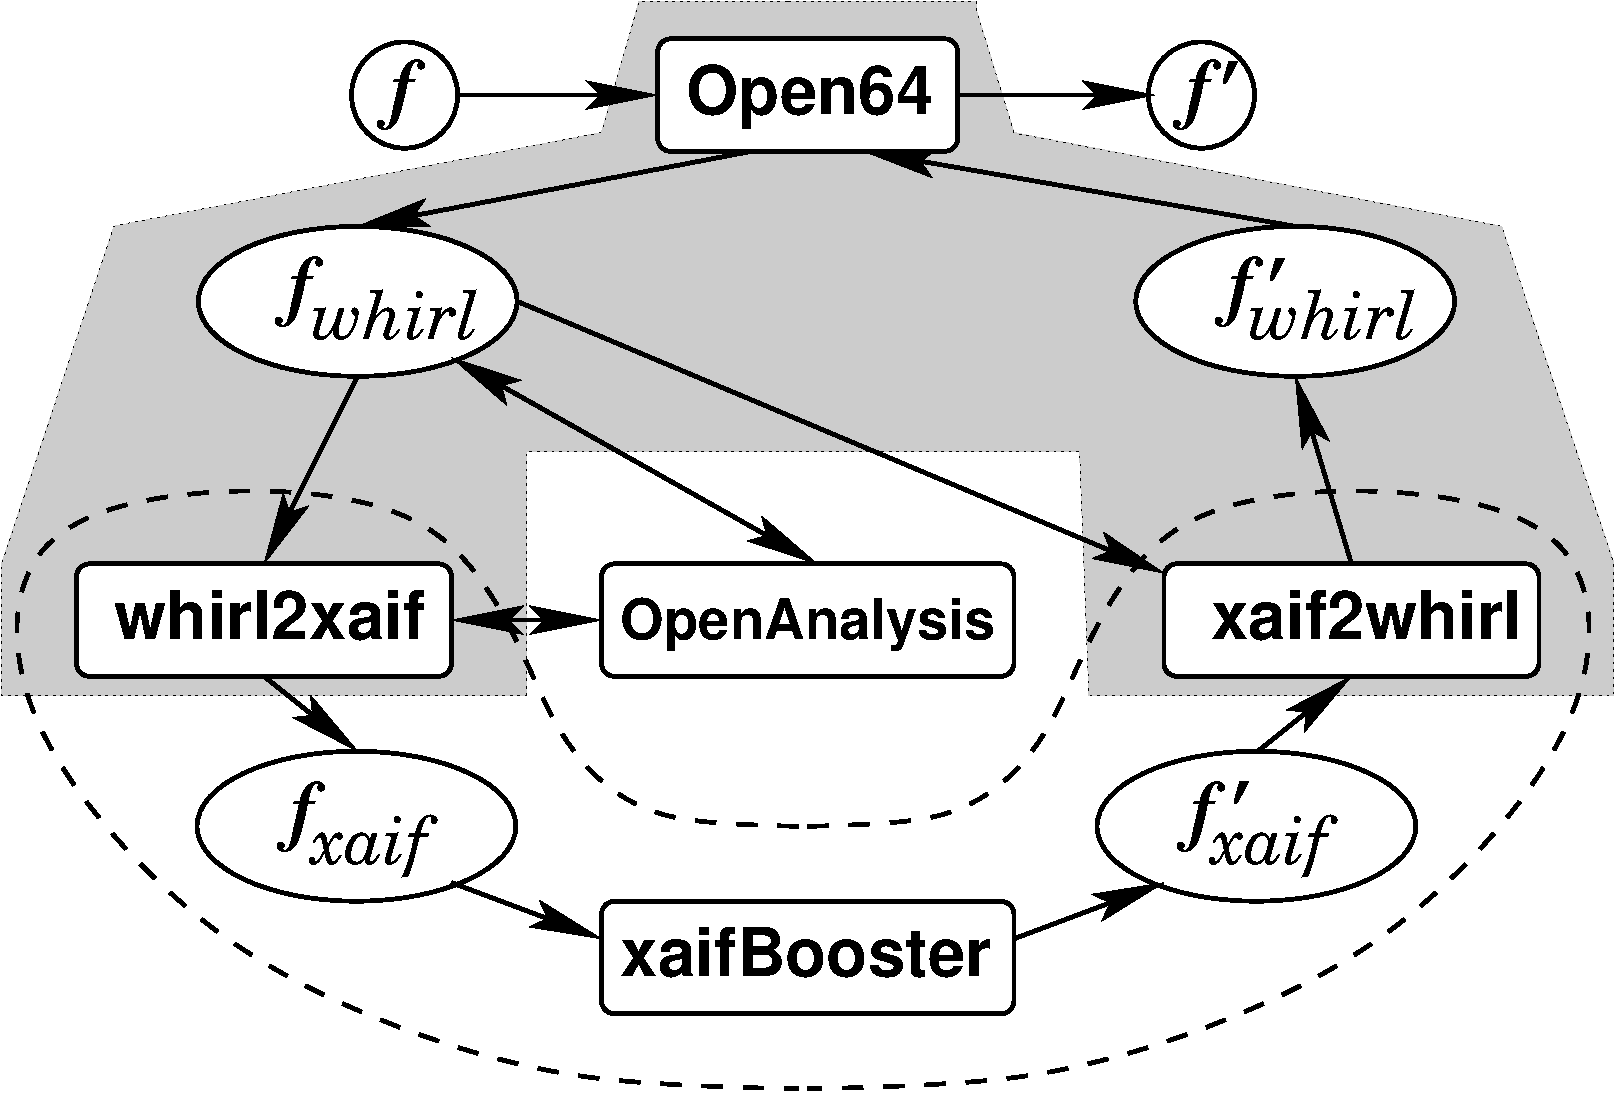
\includegraphics[width=.5\textwidth]{overview}
  \caption{\OpenADF\ components and pipeline} \label{fig:overview}
\end{figure}
\OpenADF\ has  a modular design. 
The collaboration  of the \OpenADF\ components is illustrated in 
\reffig{fig:overview}.
Our input is some numerical model given as a Fortran program 
$\bmf$.
The \OpenSixtyFour\cite{open64Web}
front-end performs a lexical, 
syntactic, and semantic analysis and produces an 
intermediate representation of $\bmf$, here denoted by $\bmf_{\whirl}$, 
in the so-called \whirl\ format.
\OpenAnalysis\ is used to build call and control flow graphs and  perform 
code analyses such as alias, activity, side-effect analysis.
This information is used by 
\whirlToxaif\ to construct a representation of the numerical core of $\bmf$ in
\xaif\ format shown as $\bmf_{xaif}$.  
A differentiated version of $\bmf_{xaif}$ is derived by an 
algorithm that is implemented in \xaifBooster\ and is again represented 
\xaif\ as $\bmfp_{xaif}$.
The information in $\bmfp_{xaif}$ and the original $\bmf_{\whirl}$ are used by 
\xaifTowhirl\ to construct a 
\whirl\ representation $\bmfp_{\whirl}$ of the differentiated code. 
The unparser of 
\OpenSixtyFour\ transforms $\bmfp_{\whirl}$ into Fortran90, thus completing
the semantic transformation of a program $\bmf$ into
a differentiated program $\bmfp$.
The gray shaded area encloses the language specific front-end that can potentially
be replaced by front-ends for languages other than Fortran. 
For instance, the new version of ADIC \cite{HoNo01} couples a C/C++ 
front-end 
based on the EDG parser \cite{edgWeb} and uses ROSE in combination with SAGE~3 \cite{roseWeb} 
as internal representation in combination with language independent components of \OpenAD.

In \refsec{chap:ADIntro} we discuss the basic concepts of AD as relevant for 
the description of \OpenAD, \refsec{chap:openadfcomponents} discusses the components 
that make up \OpenADF, and \refsec{chap:Usage} details the usage of the tool. 
Two applications further illustrate the tool usage in \refsec{chap:application} and 
we conclude with a section on future developments.

% #########################################################################################
\chapter{AD Concepts}\label{chap:ADIntro}

In this section we present the terminology and basic concepts that 
we will refer to throughout this paper. 
A detailed introduction to AD can be found in \cite{Gri00}.
The interested reader should also consider the proceedings of AD 
conferences \cite{CG91,BBCG96,CFG+01,BCH+06}.

We present the concepts and resulting transformations 
with respect to the input source code 
in a bottom up fashion.  
We first consider elemental numerical operations, 
then their control flow context within a subroutine and finally the entire program 
consisting of several subroutines in a call graph. 

We view a given numerical model as a 
vector valued function $\bmy=\bmf(\bmx): \R^n\mapsto \R^m$ that is implemented 
as a computer program in a language such as Fortran, C, or C++ and the objective is to  
compute products of Jacobians with see matrices $\bmS$.
\begin{equation}\label{eqn:JacVecProds}
\bmJ \bmS \quad \mbox{and} \quad \bmJ^T \bmS
\end{equation}
% -----------------------------------------------------------------------------------------
\section{Computational Graphs} \label{sec:computationalGraphs}

Without loss of generality we can simply assume that an evaluation of $\bmf(\bmx)$ for  
a specific value of $\bmx$ can be represented by a sequence of 
elemental operations $v_j=\phi_j(\ldots,v_i,\ldots)$. 
The $v_i$ represent the vertices $\in V$ in the corresponding computational 
graph $G=(V,E)$. The edges $(i,j)\in E$ in this graph are the direct dependencies 
$v_i\prec v_j$ implied by the elemental $v_j=\phi_j(\ldots,v_i,\ldots)$.
The elemental operations $\phi$ are differentiable on open subdomains. 
Each edge $(i,j)\in E$ has an attached local partial derivative 
$c_{ji}=\frac{\partial v_j}{\partial v_i}$. 
The central principle of AD is 
the application of the chain rule to the elemental $\phi$, that is 
multiplications and additions of the  $c_{ji}$.  

Like most of the AD literature we follow a specific numbering scheme for the vertices $v_i$.
We presume $q$ intermediate values
$v_j = \phi_j(\ldots,v_i,\ldots), v_j\in Z$
for $j=1,\ldots,q+m$ and $h,i=1-n,\ldots,q,$ $j>h,i$. 
The $n$ {\em independent}
variables $x_1,\ldots,x_n$ correspond to 
$v_{1-n},\ldots,v_0, v_i\in X$. 
We consider the 
computation of derivatives of the {\em dependent} variables 
$y_1,\ldots,y_m$ represented by $m$ variables $v_{q+1},\ldots,v_{q+m}, v_j\in Y$
with respect to the independents. 
The dependency $v_i<v_j$ implies $i<j$. 
The {\em forward mode} of AD propagates directional derivatives
as 
\begin{equation} \label{eqn:fm}
  \dot{v}_j= \sum\limits_i\frac{\partial \phi_j}{\partial v_i}\dot{v}_i 
  \quad \text{for}~~j=1,\ldots,q+m.
\end{equation} 
In {\em reverse mode} we compute adjoints of the arguments of the $\phi_j$
as a function of local partial derivatives and the 
adjoint of the variable on the left-hand side
\begin{equation} \label{eqn:rm}
  \overline{v}_i= \sum\limits_j\frac{\partial \phi_j}{\partial v_i}\overline{v}_j 
  \quad \text{for}~~j=1,\ldots,q+m.
\end{equation} 
In practice, the sum in \refeqn{eqn:rm} is often split into individual increments 
associated with each statement in which $v_i$ occurs as an argument 
$\overline{v}_i=\overline{v}_i+\overline{v}_j * \frac{\partial \phi_j}{\partial v_i}$.

Equations \refeqn{eqn:fm} and \refeqn{eqn:rm} can be used to accumulate 
the (local) Jacobian $\bmJ(G)$
of $G$, see also \refsec{sec:elimMeth}. 
% Obviously \refeqn{eqn:rm}  indicates that the dependencies of $\overline{v}_j$ and 
% $\overline{v}_i$ are reversed to those of $v_j$ and $v_i$. At the same time \refeqn{eqn:rm}
% requires all the values of the $\frac{\partial \phi_j}{\partial v_i}$ in reverse order. To make them 
% available we store them in a stack. In the  AD literature this is commonly called the {\em tape}. 

In a source transformation context we want to generate code for all $\bmf(\bmx)$
in the domain and because the above construction disregards control flow it is 
impractical here. Instead we simply consider the statements contained in a 
\basicblock\  as a section of code below the granularity of control flow and 
construct our computational (sub) graph for a \basicblock.   

% -----------------------------------------------------------------------------------------
\section{Elimination Methods} \label{sec:elimMeth}
Let $\bmf$ represent a single \basicblock\ that is subject to preaccumulation.
For notational simplicity and without loss of generality we assume that the 
dependent variables are mutually independent. 
This situation can always be
reached by introducing auxiliary assignments.
Consider the small example in \reffig{fig:toyBB}.
\begin{figure}[h]
  \begin{center}
    \begin{minipage}{.4\textwidth}
      \fontsize{8pt}{9pt}
      \verbatimfile{code/straightLine.f90}
    \end{minipage}
  \end{center}
  \caption{Example of code contained in a \basicblock}\label{fig:toyBB}
\end{figure}
Reformulating the example in terms of 
results of elemental operations $\phi$ assigned to unique intermediate 
variables $v$ we have 
\begin{equation}\label{eqn:sampleCode}
  \begin{split}
    v_1&=v_{-1}+v_0;~v_2=\sin(v_0);~v_3=v_1+v_2;~v_4=v_1*v_3; \\
    v_5&=\sqrt{v_3};~v_6=\cos(v_4);~v_7=-v_5 \quad .\\
  \end{split}
\end{equation}
In the tool this modified representation is created as part of the linearization transformation, see 
\refsec{sssec:linearization}.
In \reffig{fig:elims}~(a) we show the computational graph $G$ for this representation.
\begin{figure}
  \centering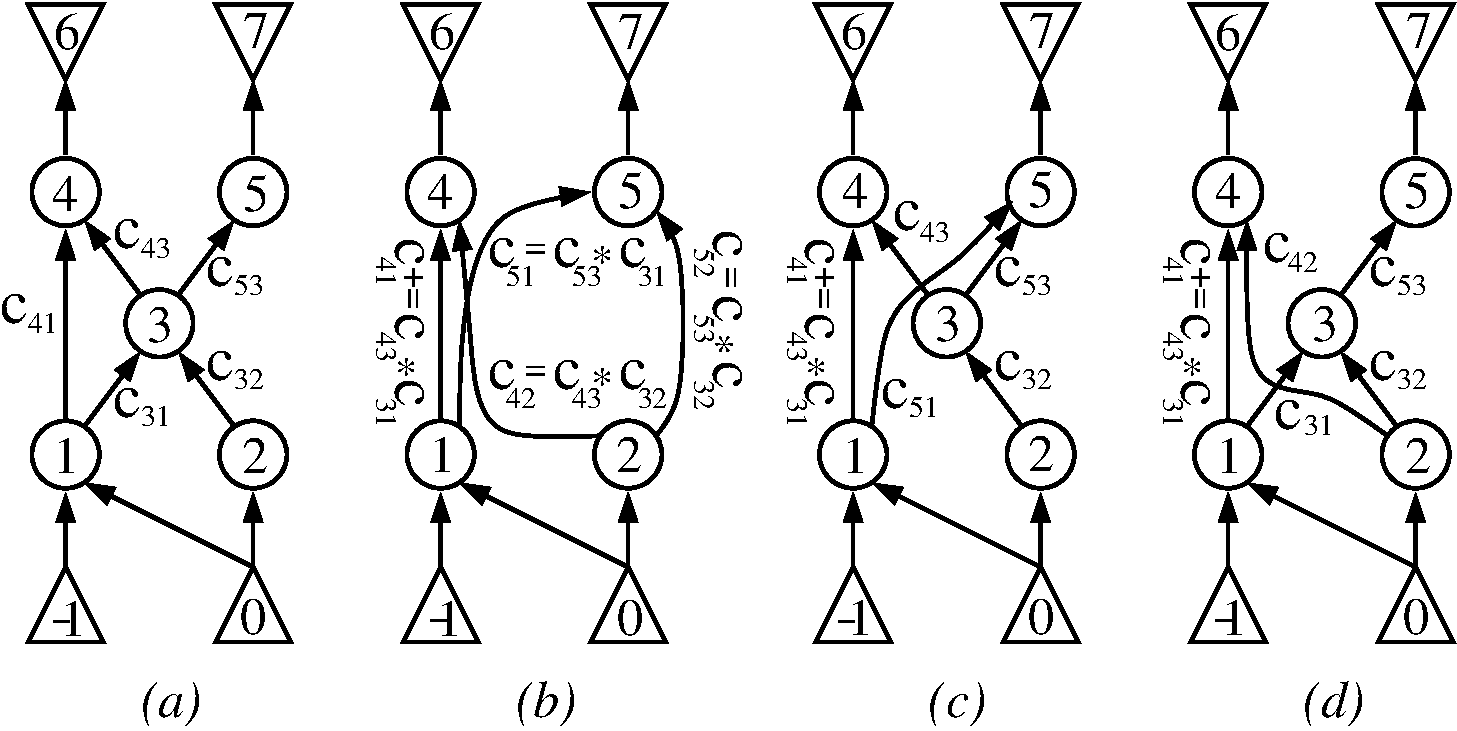
\includegraphics[width=.7\textwidth]{elims}
  \caption{
    (a) Computational graph $G$ for \refeqn{eqn:sampleCode}, 
    (b) eliminate vertex 3 from $G$, 
    (c) front eliminate edge $(1,3)$ from $G$, 
    (d) back eliminate edge $(3,4)$ from $G$} 
  \label{fig:elims}
\end{figure}
The edges $(i,j)\in E$ are labeled with partial derivatives
$c_{ji}$, for instance, in the 
example we have $c_{64}=-\sin(v_4)$.
In the tool, this graph is generated as part of the algorithm described in 
\refsec{sssec:BBPreacc}.
Jacobian preaccumulation can be interpreted as eliminations in $G$.
The graph-based elimination steps are categorized in vertex, edge, and face 
eliminations. 
In $G$ a vertex $j \in V$ is eliminated by connecting its predecessors with
its successors \cite{GrRe91}.
An edge $(i,k)$ with
$i \prec j$ and $j \prec k$ is labeled with
$c_{ki}+c_{kj} \cdot c_{ji}$ if it existed before the elimination of $j.$
We say that {\em absorption} takes place.
Otherwise, $(i,k)$ is generated as {\em fill-in} and labeled
with $c_{kj} \cdot c_{ji}$
The vertex $j$ is removed from
$G$ together with all incident edges. 
\reffig{fig:elims}~(b) shows the result of eliminating vertex $3$
from the graph in \reffig{fig:elims}~(a).

An edge $(i,j)$ is {\em front eliminated} by connecting $i$ with all successors
of $j$, followed by removing $(i,j)$ \cite{Nau00a}.
The corresponding structural modifications of the c-graph in
\reffig{fig:elims}~(a) are shown in
\reffig{fig:elims}~(c) for front elimination of $(1,3).$
The new edge labels are given as well.
Edge-front elimination eventually leads to intermediate vertices in $G$
becoming
{\em isolated}; that is, these vertices no longer have predecessors.
Isolated vertices are simply removed from $G$ together
with all incident edges.

Back elimination of an edge
$(i,j) \in E$ results in connecting all predecessors of $i$
with $j$ \cite{Nau00a}.
The edge $(i,j)$ itself is removed from $G.$
The back elimination of $(3,4)$ from the graph in \reffig{fig:elims}~(a) 
is illustrated in \reffig{fig:elims}~(d). 
Again, vertices can become isolated as a result of edge-back elimination
because they no longer have successors.
Such vertices are removed from $G.$

Numerically the elimination is the application of 
the chain rule, that is, a sequence of {\em fused-multiply-add} (fma) operations
\begin{equation}\label{eqn:fma}
  c_{ki}=c_{ji}*c_{kj}\hspace*{1ex}(+c_{ki}) 
\end{equation}
where the additions in parenthesis take place only  in the case of 
absorption or otherwise fill-in is created 
as described above.

Aside from special cases a single vertex or edge elimination will result in more
than one fma. {\em Face elimination} was introduced 
as the elimination operation with the finest granularity of exactly 
one multiplication\footnote{Additions are not necessarily directly coupled.} 
per elimination step.

Vertex and edge elimination steps have an 
interpretation in terms of vertices and edges
of $G$, whereas face elimination is performed on 
the corresponding directed line graph $\cal G.$
Following \cite{ElimTechMP}, we define the directed line graph $\cal G=(V,E)$ 
corresponding to $G=(V,E)$ as follows:
\[
{\cal V}=
\left\{\,\framebox{$i,j$}      :(i,j)\in E \right\} \cup 
\left\{\,\framebox{$\oplus,j$} :v_j  \in X \right\} \cup 
\left\{\,\framebox{$i,\ominus$}:v_i  \in Y \right\}
\] 
and 
\begin{align*}
  {\cal E}
  &=    \left\{\big(\;\framebox{$i,j$}     \,,\framebox{$j,k$}      \;\big): (i,j),(j,k) \in E        \right\} \\
  &\cup \left\{\big(\;\framebox{$\oplus,j$}\,,\framebox{$j,k$}      \;\big): v_j\in X \land (j,k)\in E\right\} \\
  &\cup \left\{\big(\;\framebox{$i,j$}     \,,\framebox{$j,\ominus$}\;\big): v_j\in Y \land (i,j)\in E\right\} 
  \quad . \\
\end{align*}
That is, 
we add a source vertex $\oplus$ and a sink vertex 
$\ominus$ to $G$ connecting all independents to $\oplus$
and all dependents to $\ominus$. $\cal G$ has   
a vertex $ v \in \cal V$ for each edge in the extended $G$, 
and $\cal G$ has an edge $ e \in \cal E$ for each 
pair of adjacent edges in $G$. \reffig{fig:face_elims} gives an 
example of constructing the directed line graph in (b) from the graph in (a) 
which is the graph from \reffig{fig:elims}(a) extended by the source and sink vertex.   
All intermediate vertices $\framebox{$i,j$} \in \cal V$ inherit the labels  
$c_{ji}$. In order to formalize face elimination, it is advantageous to move away
from the double-index notation and use one that is based on a topological
enumeration of the edges in $G.$ Hence, ${\cal G}=({\cal V}, {\cal E})$ 
becomes a DAG with ${\cal V} \subset I\!\!N$ and
${\cal E} \subset I\!\!N \times I\!\!N$ and
certain special properties.
The set of all predecessors of $j \in {\cal V}$ is denoted as $P_j.$ 
Similarly, $S_j$ denotes the set of its successors in $\cal G.$ 
A vertex 
$j \in \cal V$ is called {\em isolated} if either 
$P_j=\emptyset$ or
$S_j=\emptyset.$ 
Face elimination is defined in \cite{ElimTechMP}
between two incident intermediate vertices $i$ and $j$ in $\cal G$ as follows:
\begin{enumerate}
\item If there exists a vertex $k \in \cal V$ such that $P_k = P_i$ and
  $S_k = S_j,$ then
  set $c_k = c_k + c_j c_i$ {\em (absorption)};
  else ${\cal V}={\cal V} \cup \{k'\}$ with a new vertex $k'$ such that
  $P_{k'} = P_i$ and $S_{k'} = S_j$
  {\em (fill-in)} and labeled with $c_{k'} = c_j c_i.$
\item Remove $(i,j)$ from $\cal E.$
\item Remove $i \in \cal V$ if it is isolated. Otherwise, if there exists a vertex $i' \in \cal V$ such that
  $P_{i'} = P_i$ and $S_{i'} = S_i,$ then
  \begin{itemize}
  \item set $c_i=c_i + c_{i'}$ {\em (merge)};
  \item remove $i'.$
  \end{itemize}
\item Repeat Step 3 for $j \in \cal V.$
\end{enumerate}
In \reffig{fig:face_elims}~(c) we show the elimination of $(i,j) \in \cal E$,
where $i=\framebox{$1,3$}$ and $j=\framebox{$3,4$}$.

\begin{figure}
  \centering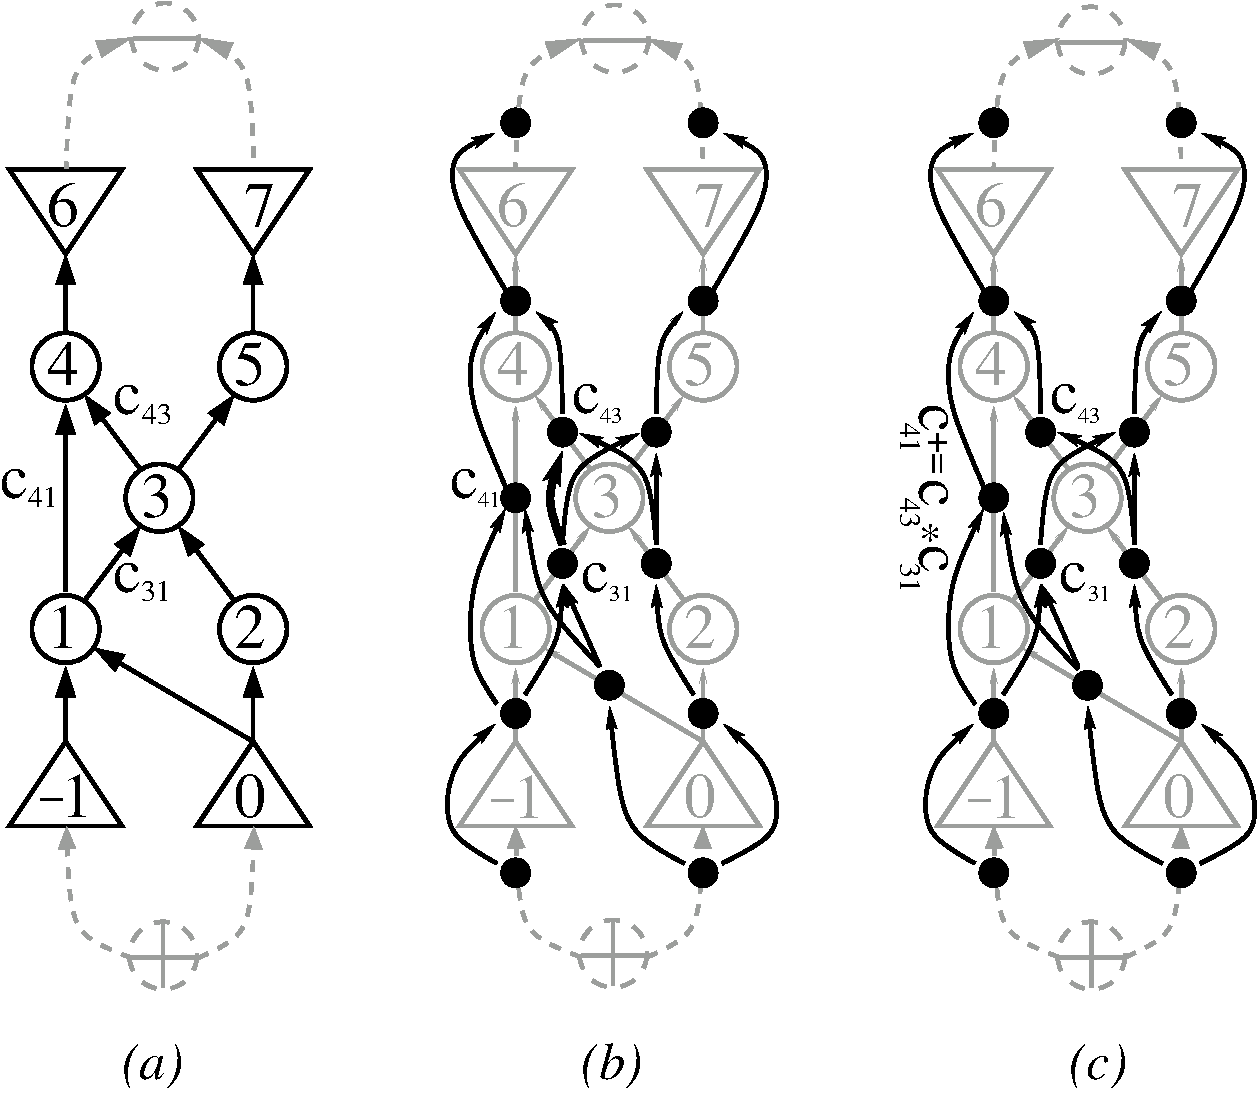
\includegraphics[width=.65\textwidth]{face_elims}
  \caption{
    (a) $G$ extended, 
    (b) $\cal G$ overlaid, 
    (c) face elimination 
  }
  \label{fig:face_elims}
\end{figure}
A complete face elimination sequence $\sigma_f$ yields a tripartite 
directed line graph $\sigma_f({\cal G})$ that can be transformed back into 
the bipartite graph representing the Jacobian $\bmfp$.
We note that any $G$ can be transformed into the 
corresponding $\cal G$ but that a back transformation 
generally is not  possible once face elimination steps have been applied. 
Therefore, face eliminations can generally not precede vertex and edge 
eliminations.
In \OpenAD\ these eliminations are implemented in the algorithms described in 
\refsec{sssec:MMTradeOff} and \refsec{sssec:angel}.

In a source transformation context of \OpenADF\ the operations \refeqn{eqn:fma} are 
expressed as actual code, the Jacobian accumulation code. For our example code 
from \reffig{fig:toyBB} the code computing 
the local partials in conjunction with the function value 
is shown in 
\reffig{fig:toyAndPartials}.
\footnote{
  For better readability we write the indices of the $c_{ji}$ with commas.
} 
\begin{figure}
  \begin{center}
    \begin{minipage}{.3\linewidth}
      \begin{align*}
        v_1&=v_{-1}+v_0; \\
        v_2&=\sin(v_0); \\
        v_3&=v_1+v_2; \\
        v_4&=v_1*v_3; \\
        v_5&=\sqrt{v_3};\\
        v_6&=\cos(v_4); \\
        v_7&=-v_5;
      \end{align*}
    \end{minipage}
    \begin{minipage}{.3\linewidth}
      \begin{align*}
        c_{1,-1}&=1; \\
        c_{2,0}&=\cos(v_0); \\
        c_{3,1}&=1; \\
        c_{4,1}&=v_3; \\
        c_{5,3}&=(2\sqrt{v_3})^{-1}; \\
        c_{6,4}&=-\sin(v_4); \\
        c_{7,5}&=-1;
      \end{align*}
    \end{minipage}
    \begin{minipage}{.2\linewidth}
      \begin{align*}
        c_{1,0}&=1; \\
        &\\
        c_{3,2}&=1; \\
        c_{4,3}&=v_1; \\
        &\\
        &\\
        &
      \end{align*}
    \end{minipage}
  \end{center}	
  \caption{Pseudo code for \refeqn{eqn:sampleCode} and the computation of the $c_{ji}$}\label{fig:toyAndPartials}
\end{figure}
In \OpenADF\ the operations in \reffig{fig:toyAndPartials} are generated by the 
transformation algorithm discussed in \refsec{sssec:linearization}.
The operations induced by the eliminations on the graph can 
be expressed in terms of the auxiliary variables $c_{ji}$.
For our example, a forward vertex elimination in the order  (1,2,3,4,5) 
in $G$ (\reffig{fig:elims}), leads to the
following Jacobian accumulation code.
\begin{figure}[h]
  % \begin{minipage}{\linewidth}
  %   \begin{align*}
  %     1:\quad  &c_{3,-1}=c_{3,1} * c_{1,-1};~c_{3,0}=c_{3,1} * c_{1,0};~c_{4,-1}=c_{4,1} * c_{1,-1};~c_{4,0}=c_{4,1} * c_{1,0}; \\
  %     2:\quad  &c_{3,0}=c_{3,2} * c_{2,0}+c_{3,0}; \\
  %     3:\quad  &c_{4,-1}=c_{4,3} * c_{3,-1}+c_{4,-1};~c_{4,0}=c_{4,3} * c_{3,0}+c_{4,0};~c_{5,-1}=c_{5,3} * c_{3,-1}; \\
  %     &c_{5,0}=c_{5,3} * c_{3,0}; \\
  %     4:\quad  &c_{6,-1}=c_{6,4} * c_{4,-1};~c_{6,0}=c_{6,4} * c_{4,0}; \\
  %     5:\quad  &c_{7,-1}=c_{7,5} * c_{5,-1};~c_{7,0}=c_{7,5} * c_{5,0} \quad .
  %   \end{align*}
  % \end{minipage}
  \begin{tabular}{l@{\hspace{1ex}}r@{\hspace{0.1ex}}l@{\hspace{1ex}}l@{\hspace{1ex}}l}
    1: &$c_{3,-1}$&$=c_{3,1} * c_{1,-1};         $&$c_{3,0}=c_{3,1} * c_{1,0};        $&$c_{4,-1}=c_{4,1} * c_{1,-1};$\\
    &$c_{4,0} $&$=c_{4,1} * c_{1,0};          $&                                    &                              \\
    2: &$c_{3,0} $&$=c_{3,2} * c_{2,0}+c_{3,0};  $&                                    &                              \\
    3: &$c_{4,-1}$&$=c_{4,3} * c_{3,-1}+c_{4,-1};$&$c_{4,0}=c_{4,3} * c_{3,0}+c_{4,0};$&$c_{5,-1}=c_{5,3} * c_{3,-1};$\\
    &$c_{5,0} $&$=c_{5,3} * c_{3,0};          $&                                    &                              \\
    4: &$c_{6,-1}$&$=c_{6,4} * c_{4,-1};         $&$c_{6,0}=c_{6,4} * c_{4,0};        $&                              \\
    5: &$c_{7,-1}$&$=c_{7,5} * c_{5,-1};         $&$c_{7,0}=c_{7,5} * c_{5,0};        $&            
  \end{tabular}
  \caption{Pseudo code for vertex eliminations for \refeqn{eqn:sampleCode}}\label{fig:toyAccumulation}
\end{figure}
In the tool the operations shown in \reffig{fig:toyAccumulation} are generated by the 
transformation algorithm discussed in \refsec{sssec:BBPreacc}. 

% -----------------------------------------------------------------------------------------
\section{Control Flow Reversal} \label{sec:cfReversal}
Because the code for a $\bmf$ generally contains control flow constructs there is no 
single  computational graph 
$G$ that represents the computation of $\bmf$ for all possible values of $\bmx$.
We explained in \refsec{sec:computationalGraphs} that \OpenADF\ considers subgraphs constructed 
from the contents of a \basicblock.
In the example shown in \reffig{fig:toy} we put the \basicblock\ code shown in 
\reffig{fig:toyBB} into a control flow context, see lines 06--09.
\begin{figure}
  \begin{center}
    \begin{minipage}{.5\textwidth}
      \begin{tabbing}
        \hspace{.6cm}{\footnotesize \bf 00}\hspace{.5cm} {\tt y(k) = sin(x(1)*x(2))} \\
        \hspace{.6cm}{\footnotesize \bf 01}\hspace{.5cm} {\tt k    = k+1} \\
        \hspace{.6cm}{\footnotesize \bf 02}\hspace{.5cm} {\tt if} \={\tt (mod(k,2) .eq. 1) then } \\
        \hspace{.6cm}{\footnotesize \bf 03}\hspace{.5cm} \>{\tt y(k) = 2*y(k-1)}  \\
        \hspace{.6cm}{\footnotesize \bf 04}\hspace{.5cm} {\tt else } \\
        \hspace{.6cm}{\footnotesize \bf 05}\hspace{.5cm} \>{\tt do} \={\tt i=1,k } \\
        \hspace{.6cm}{\footnotesize \bf 06}\hspace{.5cm} \>\>{\tt t1   = x(1)+x(2) } \\
        \hspace{.6cm}{\footnotesize \bf 07}\hspace{.5cm} \>\>{\tt t2   = t1+sin(x(1)) } \\
        \hspace{.6cm}{\footnotesize \bf 08}\hspace{.5cm} \>\>{\tt x(1) = cos(t1*t2) } \\
        \hspace{.6cm}{\footnotesize \bf 09}\hspace{.5cm} \>\>{\tt x(2) = -sqrt(t2) } \\
        \hspace{.6cm}{\footnotesize \bf 10}\hspace{.5cm} \>{\tt end do } \\
        \hspace{.6cm}{\footnotesize \bf 11}\hspace{.5cm} {\tt end if } \\
        \hspace{.6cm}{\footnotesize \bf 12}\hspace{.5cm} {\tt y(k) = y(k)+x(1)*x(2) } 
      \end{tabbing}
    \end{minipage}
  \end{center}
  \caption{Toy example code with control flow}\label{fig:toy}
\end{figure}
The control flow graph (CFG) \cite{ASU86} resulting from the above code is depicted in 
\reffig{fig:cfg}(a).
The assignment statements are contained in the {\basicblock}s B(2,4,6,9).
For instance, 
the statements from \reffig{fig:toyBB} now  in lines 06--09 form the loop body, \basicblock\ B(6).
As B(6) is executed
\code{k} times it may be worth putting
additional effort into the optimization of the derivative code 
generated for B(6) by optimizing the elimination sequence as illustrated in 
\refsec{sec:elimMeth}.
\begin{figure}[ht]
  \centering
  \begin{tabular}{ccc}
    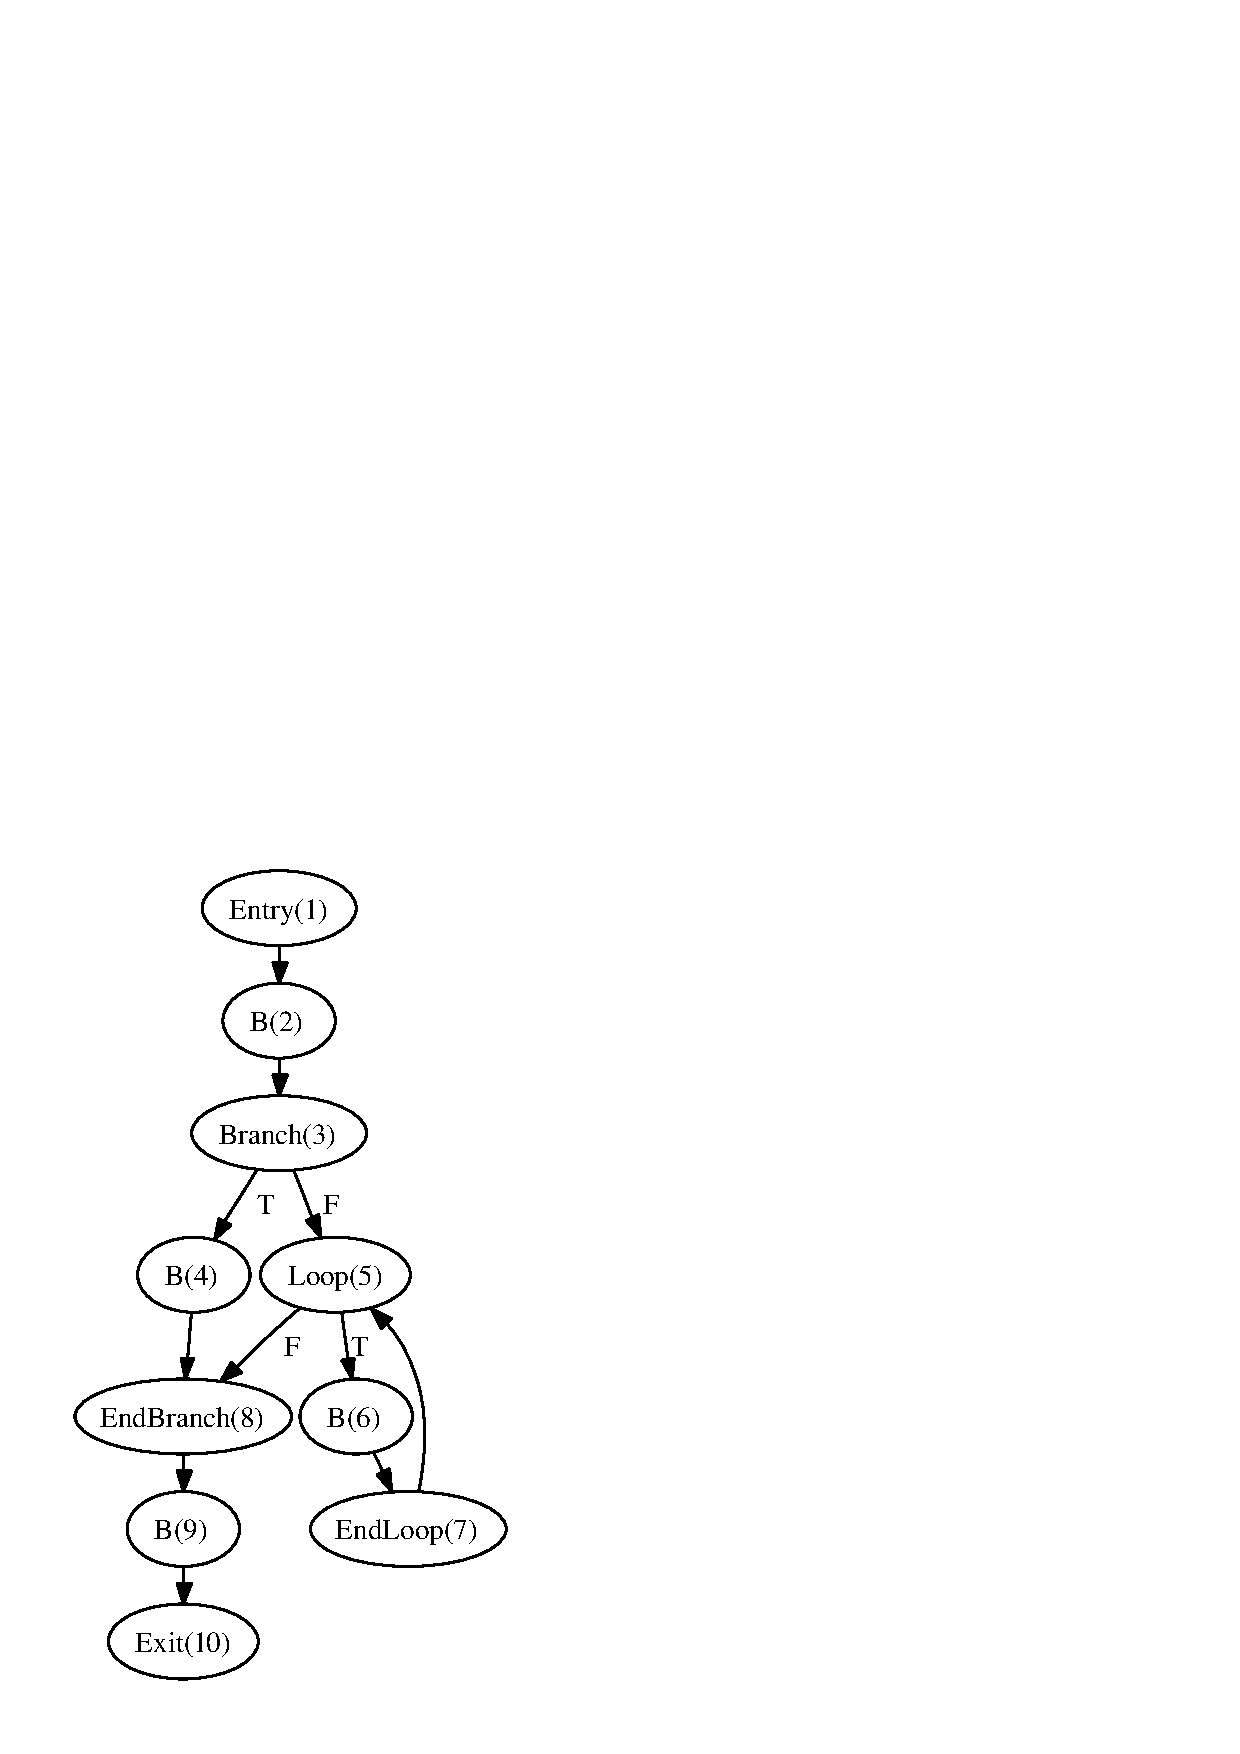
\includegraphics[width=.25\textwidth]{cfg_ts}
    &
    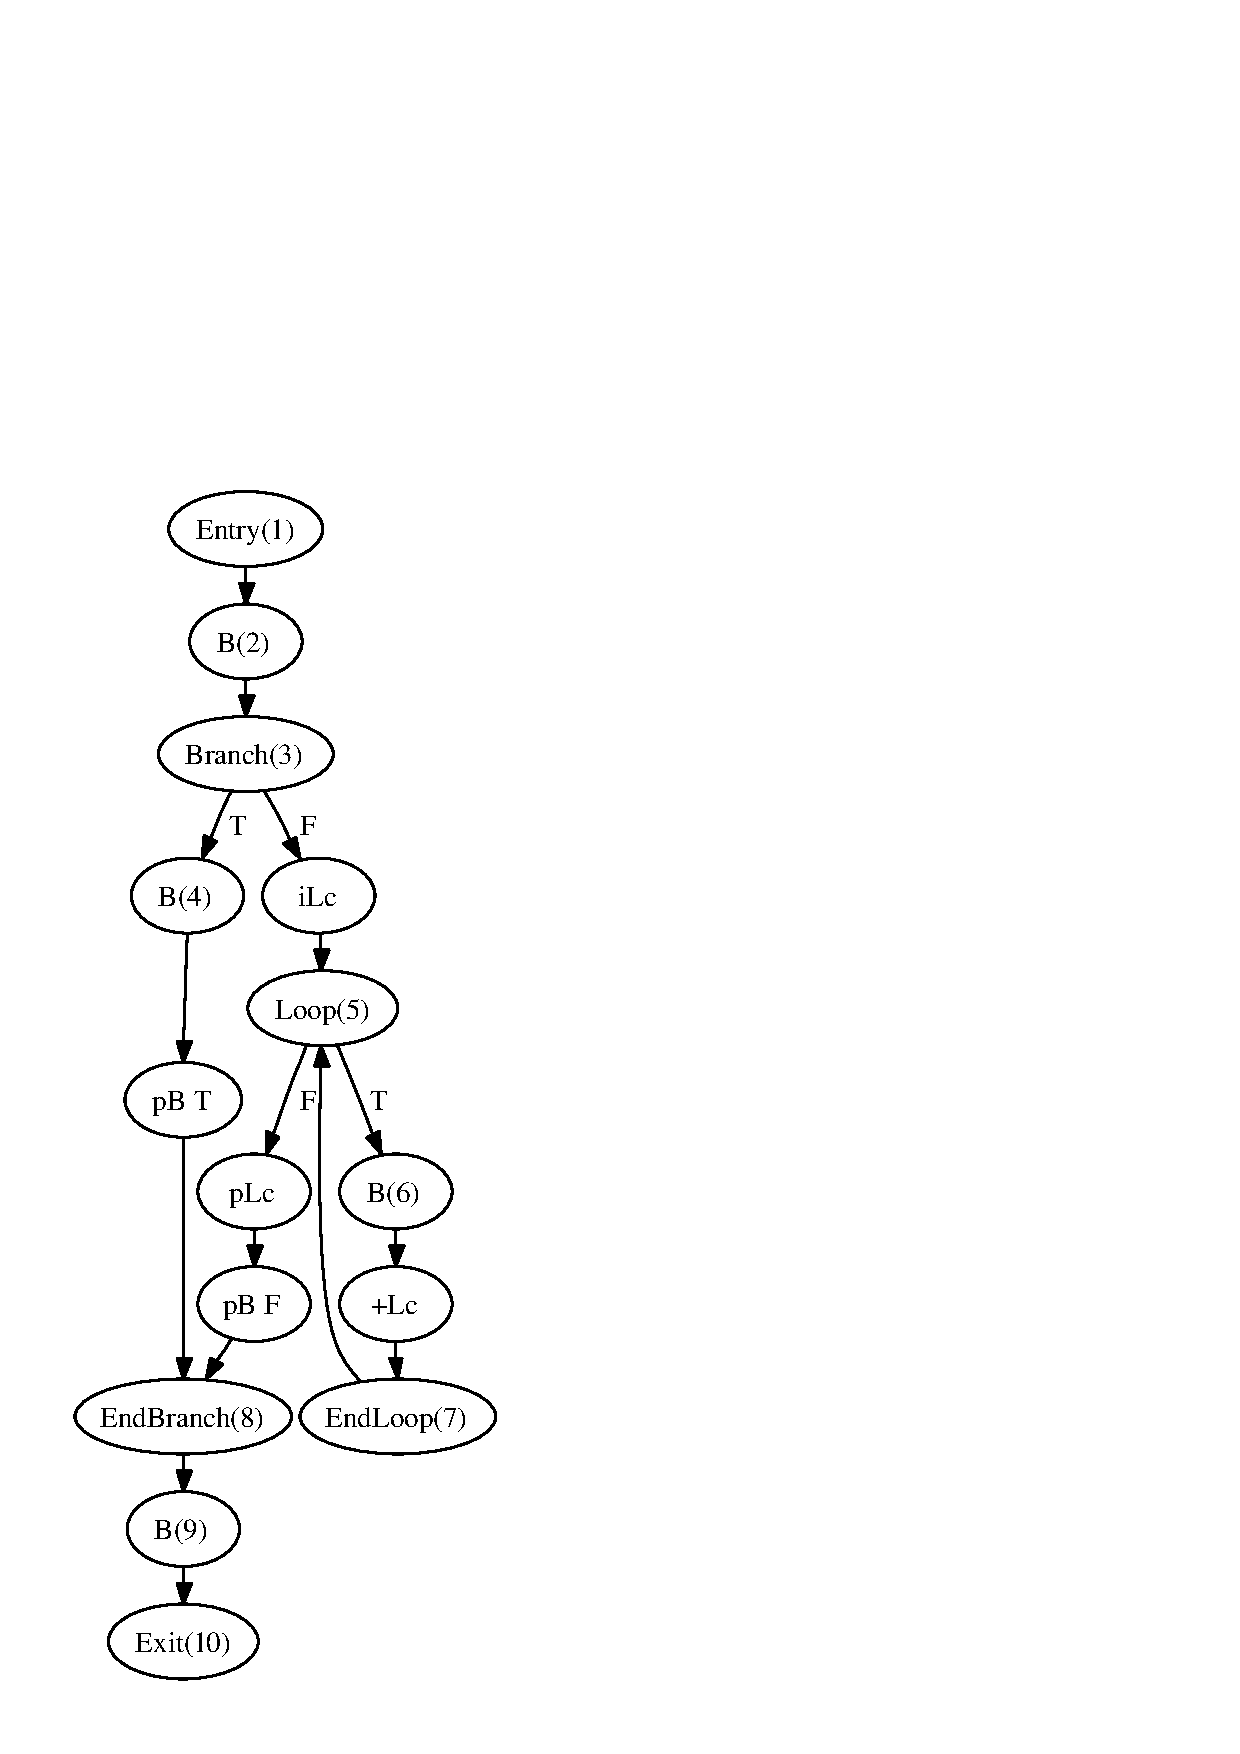
\includegraphics[width=.25\textwidth]{cfg_tape}
    &
    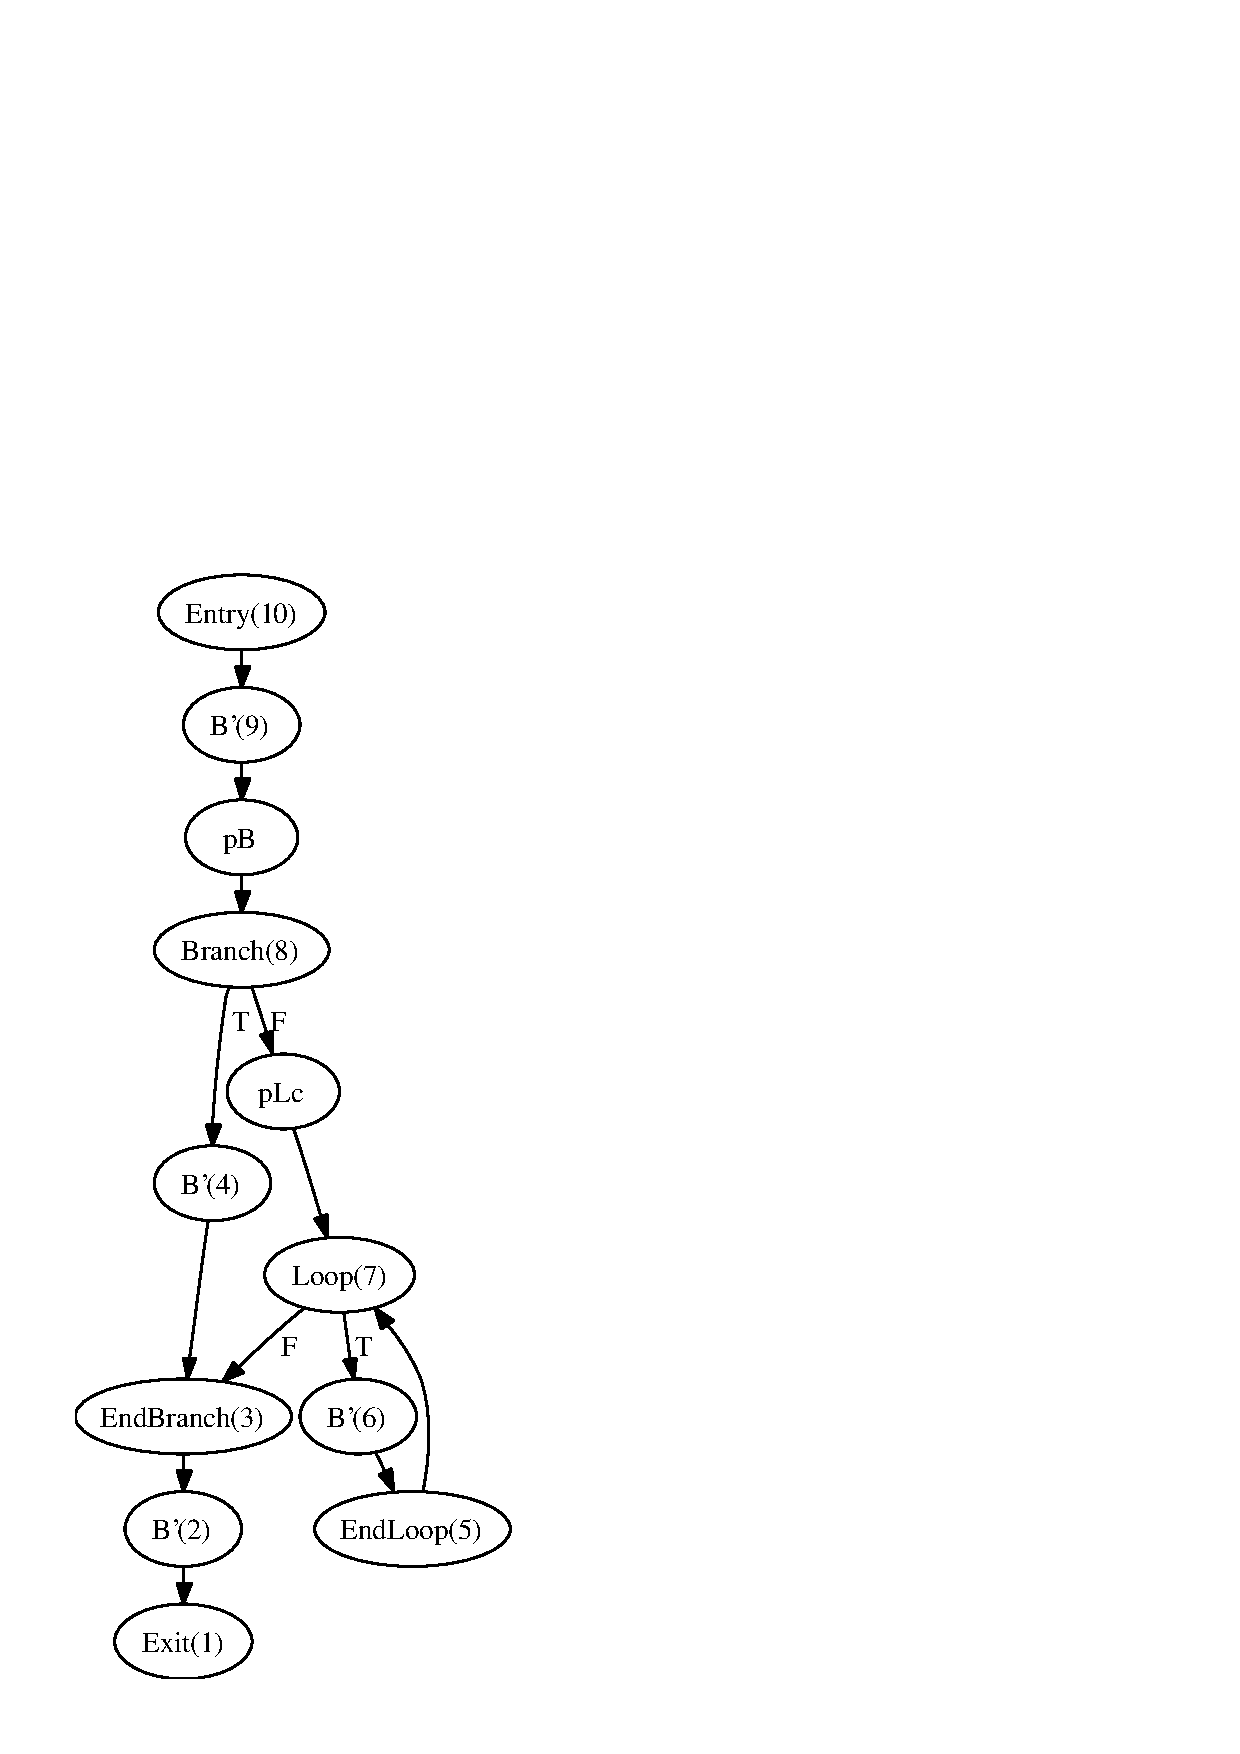
\includegraphics[width=.25\textwidth]{cfg_adj}
    \\
    \em (a) & \em (b) & \em (c)
  \end{tabular}
  \caption{CFG of \reffig{fig:toy} (a) original, (b) trace generating, (c) reversed}\label{fig:cfg}
\end{figure}
For B(6) the corresponding computational graph $G$  see 
\reffig{fig:elims}(a).  

For a sequence of $l$ {\basicblock}s that are part of 
a path through the CFG for a particular value of $\bmx$ the 
equations~(\ref{eqn:fm}) and (\ref{eqn:rm}) can be generalized as follows:
\begin{equation} \label{eqn:bbfm}
  \dot{\bmy}_j=\bmJ_j \dot{\bmx}_j \quad \text{for}~~j=1,\ldots,l
\end{equation} 
and 
\begin{equation} \label{eqn:bbrm}
  \bar{\bmx}_j=\bmJ^T_j \bar{\bmy}_j \quad \text{for}~~j=l,\ldots,1\quad ,
\end{equation} 
where $\bmx_j = (x^j_i \in V :  i=1,\ldots,n_j)$ and
$\bmy_j = (y^j_i \in V : i=1,\ldots,m_j)$ are the inputs and outputs of the 
{\basicblock}s
respectively. 
In {\em forward mode} a sequence of 
products of the local Jacobians $\bmJ_j$ 
with the directions $\dot{x}_j$ 
are propagated forward in the direction of the flow of control, for 
instance simultaneously to the computation of $\bmf$.
In our example \basicblock\ B(6) is the third \basicblock\ ($j=3$) and we have
$\bmx_3=\bmy_j=($\code{x(1)}$,$\code{x(2)}$)$ and 
consequently have the operations for the Jacobian vector product shown 
in \reffig{fig:toyPreacc}.  
\begin{figure}[h]
  \begin{center}
    \begin{align*}
      t_1&=\dot{\tt x}\mbox{\tt (1)} ; \\
      t_2&=\dot{\tt x}\mbox{\tt (2)}; \\
      \dot{\tt x}\mbox{\tt (1)}&=c_{6,-1}*t_1; \\
      \dot{\tt x}\mbox{\tt (1)}&=\dot{\tt x}\mbox{\tt (1)}+c_{6,0}*t_2; \\
      \dot{\tt x}\mbox{\tt (2)}&=c_{7,-1}*t_1; \\
      \dot{\tt x}\mbox{\tt (2)}&=\dot{\tt x}\mbox{\tt (2)}+c_{7,0}*t_2; 
    \end{align*}
  \end{center}	
  \caption{Pseudo code for $\bmJ_3\dot{\bmx}_3$ for the loop body in \reffig{fig:toy}}\label{fig:toyPreacc}
\end{figure}
Note that the code overwrites \code{x(1)} and \code{x(2)} and therefore 
we have to preserve the original derivatives in temporaries $t_1$ and $t_2$.

In {\em reverse mode} products of the transposed
Jacobians $\bmJ^T_j$ with adjoint vectors $\overline{\bmy}_j$
are propagated reverse to the direction of the flow of control.
The $\bmJ^T_j$ can be computed by augmenting the original code with 
linearization and Jacobian accumulation statements, see \refsec{sec:elimMeth}.
The preaccumulated  $\bmJ^T_j$ are stored during the forward execution
which is commonly called the {\em tape}, see \reffig{fig:toyPreaccRev}(a) for an 
example. They are retrieved from the 
tape for computing \refeqn{eqn:bbrm} during the reverse execution, see \reffig{fig:toyPreaccRev}(b) for 
an example. 
It is always possible to organize the store and retrieve such that the tape can be 
implemented as a stack.
\begin{figure}[h]
  \begin{center}
    \begin{minipage}[b]{.2\linewidth}
      \code{push(}$c_{6,-1}$\code{);}\\
      \code{push(}$c_{6,0}$\code{);}\\
      \code{push(}$c_{7,-1}$\code{);}\\
      \code{push(}$c_{7,0}$\code{);}\\
      \\ \\ \\
      \centerline{(a)}
    \end{minipage}
    \begin{minipage}[b]{.2\linewidth}
      \small
      \begin{align*}
        t_2&=\code{pop()}*\bar{\tt x}\mbox{\tt (2)};\\
        t_1&=\code{pop()}*\bar{\tt x}\mbox{\tt (2)};\\
        t_2&=t_2+\code{pop()}*\bar{\tt x}\mbox{\tt (1)};\\
        t_1&=t_1+\code{pop()}*\bar{\tt x}\mbox{\tt (1)};\\
        \bar{\tt x}\mbox{\tt (2)}& =t_2;\\
        \bar{\tt x}\mbox{\tt (1)}& =t_1;
      \end{align*}
      \centerline{(a)}
    \end{minipage}
  \end{center}	
  \caption{Pseudo code for writing the tape (a) and consuming the tape for  $\bmJ_3^T\bar{\bmy}_3$ (b) for  the loop body in \reffig{fig:toy}}\label{fig:toyPreaccRev}
\end{figure}

In order to find the corresponding path to the reversed control flow graph 
we also have to generate a trace which is done with an augmented CFG,
for our toy example see \reffig{fig:cfg}(b).
This augmented CFG  keeps track of which branch was taken and counts how 
often a loop was 
executed.  
This information is pushed on  a stack and popped from that stack during the 
reverse sweep see also \cite{NULF04CFR}. Because the control flow trace 
adheres to the stack model it often is also considered part of the tape. 
In the example in \reffig{fig:cfg}(b) the extra {\basicblock}s pBT and pBF push 
a boolean (T or F) onto the stack depending on the branch. 
In iLc we initialize a loop counter, increment the loop counter in +Lc, 
and push the final count in pLc. 

\reffig{fig:cfg}(c) shows the reversed CFG for our toy example. 
The parenthesized numbers in the node labels align the 
node transformation to \reffig{fig:cfg}(a). 
The \exit\ node becomes 
the \entry, \Loop\ becomes \EndLoop, \branch\ becomes \EndBranch, and vice versa. 
Each \basicblock\  B is replaced with its reversed version B'.  
Finally, to find the proper path through this reversed CFG we need to retrieve 
the information recorded in  \reffig{fig:cfg}(b). The extra nodes pB and pLc 
pop the branch information and the loop counter respectively.  
We enter the branch and execute the loop as indicated by the recorded information. 
The process of the control flow reversal is described in detail in 
\cite{NULF04CFR}. 

% -----------------------------------------------------------------------------------------
\section{Call Graph Reversal} \label{sec:cgReversal}

Generally, the computer program 
induces a {\em call graph} (CG) \cite{ASU86}
whose vertices are subroutines and whose edges 
represent calls potentially made during the computation of $\bmy$ for all 
values of $\bmx$ in the domain of $\bmf$.

For a large number of problems it is possible to statically 
predetermine either 
{\em split} or {\em joint} 
reversal \cite{Gri00} for any subroutine in the call graph .
These concepts are easier understood with the help of the dynamic call tree,
see also \cite{NaUt05STAG}.
\begin{figure}
  \centering
  \begin{tabular}{p{.5\linewidth}p{.3\linewidth}}
    \begin{minipage}[b]{\linewidth}
      \footnotesize
      \tt subroutine A()\\
      \hspace*{3ex}call B(); call D(); call B();\\
      end subroutine A\\[.2em]
      subroutine B()\\
      \hspace*{3ex}call C()\\
      end subroutine B\\[.2em]
      subroutine C()\\
      \hspace*{3ex}call E()\\
      end subroutine C
    \end{minipage}
    &
    \vspace*{-3.2cm}
    \centering{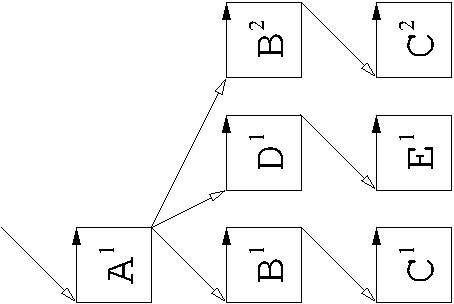
\includegraphics[width=3.2cm,origin=c,angle=-90]{edct_ns}}
  \end{tabular}
  \caption{Dynamic call tree of a simple calling hierarchy}
  \label{fig:simple_dct}
\end{figure}
where each vertex represents an actual invocation of a subroutine for a 
given execution of the program, see \reffig{fig:simple_dct} and 
\reftab{tab:leg} for an explanation of the symbols. 
The order of calls is implied by following the edges in left to right order. 
Using split reversal for all subroutines in the  program 
means that first the tape for the entire program is written. Then 
we follow with the reverse steps that read the tape, see \reffig{fig:split}. 

\begin{table}[t]
  \begin{center}
    \begin{tabular}{clcl}
      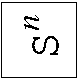
\includegraphics[origin=c,angle=-90,width=0.7cm]{box}  
      & 
      \begin{minipage}[b]{.3\linewidth}
        $n$-th invocation
        of subroutine {\tt S}
      \end{minipage} 
      & 
      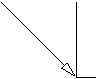
\includegraphics[origin=c,angle=-90,width=0.7cm]{call} & 
      \begin{minipage}[b]{.3\linewidth}
        subroutine call\\[-2mm]
      \end{minipage} 
      \\ 
      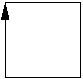
\includegraphics[origin=c,angle=-90,width=0.7cm]{rf}  & 
      \begin{minipage}[b]{.3\linewidth}
        run forward \\[-2mm]
      \end{minipage}
      & 
      
\includegraphics[origin=c,angle=-90,width=0.7cm]{order}  & 
      \begin{minipage}[b]{.3\linewidth}
        order of execution \\[-2mm]
      \end{minipage}
      \\
      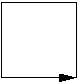
\includegraphics[origin=c,angle=-90,width=0.7cm]{sac}  & 
      \begin{minipage}[b]{.3\linewidth}
        store checkpoint \\[-2mm]
      \end{minipage}
      & 
      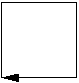
\includegraphics[origin=c,angle=-90,width=0.7cm]{rac}  & 
      \begin{minipage}[b]{.3\linewidth}
        restore checkpoint \\[-2mm]
      \end{minipage}
      \\
      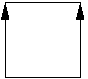
\includegraphics[origin=c,angle=-90,width=0.7cm]{ta}  & 
      \begin{minipage}[b]{.3\linewidth}
        run forward and tape \\[-2mm]
      \end{minipage}
      & 
      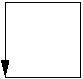
\includegraphics[origin=c,angle=-90,width=0.7cm]{ad}  & 
      \begin{minipage}[b]{.3\linewidth}
        run adjoint \\[-2mm]
      \end{minipage}
      \\
    \end{tabular}
  \end{center}
  \vspace*{-.5cm}
  \caption{Symbols for call tree reversal}
  \label{tab:leg}
\end{table}

\begin{figure}[t]
  \centerline{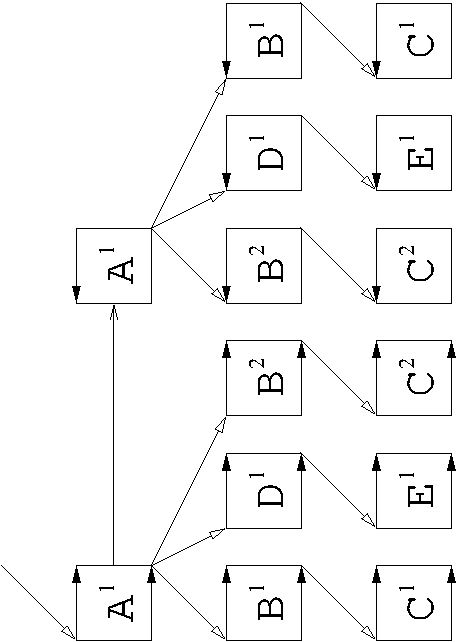
\includegraphics[width=3.2cm,origin=c,angle=-90]{edct_split_ns}}
  \vspace*{-.5cm}
  \caption{Dynamic call tree for split reversal}
  \label{fig:split}
\end{figure}

\begin{figure}[t]
  \centerline{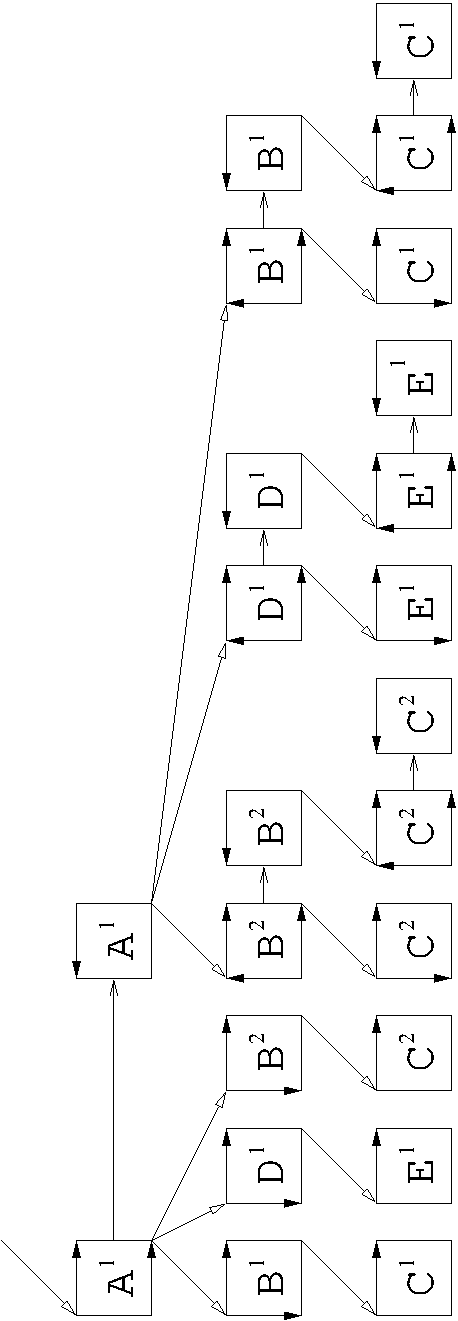
\includegraphics[width=3.2cm,origin=c,angle=-90]{edct_joint_ns}}
  \vspace*{-3cm}
  \caption{DCT of adjoint obtained by joint reversal mode}
  \label{fig:joint}
\end{figure}

Using joint reversal for all subroutines in a program 
means that the tape, see \refsec{sec:cfReversal} for a each 
subroutine invocation is written immediately before the reverse execution for 
that invocation. In our example this implies that we have to generate 
a tape for {\tt C}$^2$ while the caller {\tt B}$^2$ is being reversed, 
i.e. this is not the proper context to simply reexecute {\tt C}$^2$. 
We can either reexecute the entire program up to the  {\tt C}$^2$
call and then start taping, or (preferably) we store the arguments while 
running forward and restore them before starting the taping. 
The ensuing dynamic call tree for our example is 
shown in \reffig{fig:joint}. 
For many applications neither an all split nor all joint reversal
is efficient. Often a mix of split and joint reversals statically  
applied to subtrees of the call tree is suitable.  

% #########################################################################################
\chapter{Components of \OpenADF}\label{chap:openadfcomponents}

\OpenADF\ is built on components that belong to a framework designed
for code transformation of numerical programs.  The components are
tied together either via programmatic interfaces or by communication
using the \xaif\ language. The transformation of the source code follows the
pipeline shown in \reffig{fig:overview}.  
In \refsec{sec:openadcomponents} we describe the language-independent 
components of \OpenAD\ framework and \refsec{sec:fortfe} provides details 
in the Fortran front-end.
The regular setup procedure for \OpenADF, see also \refsec{sec:dab}, 
will retrieve all components into an \code{OpenAD/} directory to which 
we refer from here on.  

% -----------------------------------------------------------------------------------------
\section{Language Independent Components (\OpenAD)}\label{sec:openadcomponents}

The component design of the tool aims for reuse of the different components 
for different types of source transformation of numerical codes, for 
different programming languages in which these tools are written and finally 
also for the reuse of the individual components in different contexts. 
A second, equally important concern is the flexibility of the tool.  
This section covers the language independent components that make up the core \OpenAD\ framework. 

% -----------------------------------------------------------------------------------------
\subsection{Static Code Analyses (\OpenAnalysis)} \label{ssec:openanalysis}

The \OpenAnalysis\ toolkit, see \cite{oaWeb}, separates program
analysis from language-specific or front-end specific intermediate
representations.  This separation enables a single implementation of
domain-specific analyses such as activity analysis, to-be-recorded
analysis, and linearity analysis in \OpenADF.  Standard analyses
implemented within \OpenAnalysis\ such as CFG construction, call graph
construction, alias analysis, reaching definitions, ud- and du-chains,
and side-effect analysis are also available via
\OpenADFortTk.

\OpenADFortTk\ interfaces with \OpenAnalysis\ as a producer and a
consumer.  A description of Alias analysis illustrates this
interaction.  \xaif\ requires an alias map data structure, in which
each variable reference is mapped to a set of virtual locations that
it may or must reference.  For example, if a global variable \code{g}
is passed into subroutine \code{foo} through the reference parameter
\code{p}, variable references \code{g} and \code{p} will reference the
same location within the subroutine \code{foo} and therefore be aliases.  
\OpenAnalysis\ determines the aliasing relationships by querying an
abstract interface called the alias IR interface, which is a 
language-independent interface between \OpenAnalysis\ and any
intermediate representation for an imperative programming language.  
An implementation of the alias IR interface for the Fortran~90
intermediate representation is part of
\OpenADFortTk.  The interface includes queries for an iterator over
all the procedures, statements in those procedures, memory references
in each statement, and memory reference expression and location
abstractions that provide further information about memory references
and symbols.  The results of the alias analysis are then provided back
to \OpenADFortTk\ through an alias results interface.

Using language-independent interfaces between \OpenAnalysis\ and the
intermediate representation will enable alias analysis for multiple
language front-ends without requiring \xaif\ to include the union of
all language features that affect aliasing (ie. pointer arithmetic and
casting in C/C++ and equivalence in Fortran~90).  Instead
\OpenAnalysis\ has analysis-specific interfaces for querying
language-specific intermediate representations.

\OpenAnalysis\ also performs activity analysis.  For activity analysis
the independent and dependent variables of interest are communicated
to the front-end through the use of pragmas, see \refsec{sssec:mfef}.
The results of the analysis are then encoded by the Fortran~90
front-end into \xaif.  The analysis indicates which variables are
active at any time, which memory references are active, and which
statements are active.

The activity analysis itself is based on the formulation in~\cite{HNP02}.
The main difference is that the data-flow framework in \OpenAnalysis\ does not
yet take advantage of the structured data-flow equations.  Activity analysis is
implemented in a context-insensitive, flow-sensitive interprocedural fashion.

All sources for \OpenAnalysis\ can be found under \code{OpenAD/OpenAnalysis/}.

% -----------------------------------------------------------------------------------------
\subsection{Representing the Numerical Core (\xaif)} \label{ssec:xaif}

To obtain a language independent representation of programs across multiple 
programming languages one might choose the union of all language features. 
On the other hand one can observe that the majority of differences between 
languages does not lie with the elemental numerical operations that are at the 
heart of AD transformations. This more narrow representation 
is a compromise permitting just enough coverage to achieve language 
independence for the numerical core across languages.
Consequently, certain program features are not represented and have 
to be retained by the language specific front-end to reassemble the 
complete program from the (transformed) numerical core.
Among the generic language features not considered part of the numerical core are: 
\begin{itemize}
  \parskip = -2pt
\item user type definitions and member access, see also \refsec{sssec:Canonicalization}
\item pointer arithmetic
\item I/O operations  
\item memory management, see also \refsec{chap:concl}
\item preprocessor directives
\end{itemize}
For a more general discussion regarding this compromise see also \cite{UtNa04SLD}.
It is apparent that certain aspects of the adjoint code such as 
checkpointing, see \refsec{sec:cgReversal}, and taping, see \refsec{sec:cfReversal},
can involve memory allocation and various I/O schemes and therefore 
are not amenable to representation in the \xaif. 
At the same time it is also clear that the way  one has to handle the memory and I/O for 
taping and checkpointing is primarily determined by the problem size at runtime and not
primarily by the code we transform.   
Therefore in \OpenAD\ such transformation results are handled by  specific 
code expansion for subroutine specific templates and inlinable subroutine calls 
in the post processor, see \refsec{sssec:PostProcessor}. This not only avoids 
the typically language specific I/O and memory management aspects, it also 
affords additional flexibility.   

The format of choice in \OpenAD\ is an XML-based \cite{xmlWeb} hierarchy of 
directed graphs, referred to as \xaif 
\cite{HNN02}. Using XML is motivated by the existence of XML parsers and 
the ability to specify the \xaif\ specific XML contents with a schema which 
the parser can use to validate a given \xaif\ representation. 
The current \xaif\ schema is documented at \cite{xaifweb}.
The basic building blocks are the same data structures commonly found 
in compilers from top down call graph with scopes and symbol tables, 
control flow graphs as call graph vertices, basic blocks  as control flow 
graph vertices, statement lists contained in basic blocks, 
assignments as a statement with expression graphs,  and variable references 
and intrinsic operations as expression graph vertices. 
The role of the respective elements in the \xaif\ schema is fairly self evident. 
Elements are associated by containment. In the graph structures edges 
refer to source and target vertices by vertex ids. 
Variable references contain references to symbols which in turn 
are associated to symbol table elements via a scope and a symbol id. 
An example can be found in \refsec{sssec:wtxxtw}, \reffig{fig:exampleXaifCode}.
Further documentation for individual elements can be found directly in the 
schema annotations. 

The \xaif\ also contains the results of the code analyses provided 
by \OpenAnalysis, see \refsec{ssec:openanalysis}. Some are expressed 
either as additional attributes on certain \xaif\ elements, e.g. for activity information. 
Side-effect analysis provides lists of variable references per subroutine, i.e. a call graph vertex element.
DuUd chains are expressed as list of ids found in the assignment \xaif\ element.
Alias information is expressed as set of virtual addresses. 
DuUd chains and alias information is collected in maps indexed by keys associated with the call 
graph. References to individual entries held in these maps are expressed via foreign key 
attributes in the elements. 

The source transformation at the code of \OpenAD\ potentially changes and augments 
all elements of the \xaif. While it would in principle be possible  
to express the result entirely in the plain \xaif\ format we already mentioned the 
code expansion approach. Therefore the transformed \xaif\ adheres to a schema 
that is extended by a construct to represent inlinable subroutine calls and 
a specific list of control flow graphs that the post processor places in predefined 
locations in the subroutine template.    

The \xaif\ schema and examples can be found under \code{OpenAD/xaif/}.

% -----------------------------------------------------------------------------------------
\subsection{Transforming the Numerical Core (\xaifBooster)} \label{sssec:xaifBooster}
The transformation engine that differentiates the \xaif\ representation of 
$\bmf$ is called \xaifBooster. It is implemented in C++ based on a 
data structure that represents all information supplied in the \xaif\ input 
together with collection of algorithms that operate on this data structure, modify 
it and produce transformed \xaif\ output as the result. All sources for \xaifBooster\ can be found under \code{OpenAD/xaifBooster/}. The principal setup of the source tree is shown in \reftab{tab:dirStruct}.
\begin{figure}
  \centering 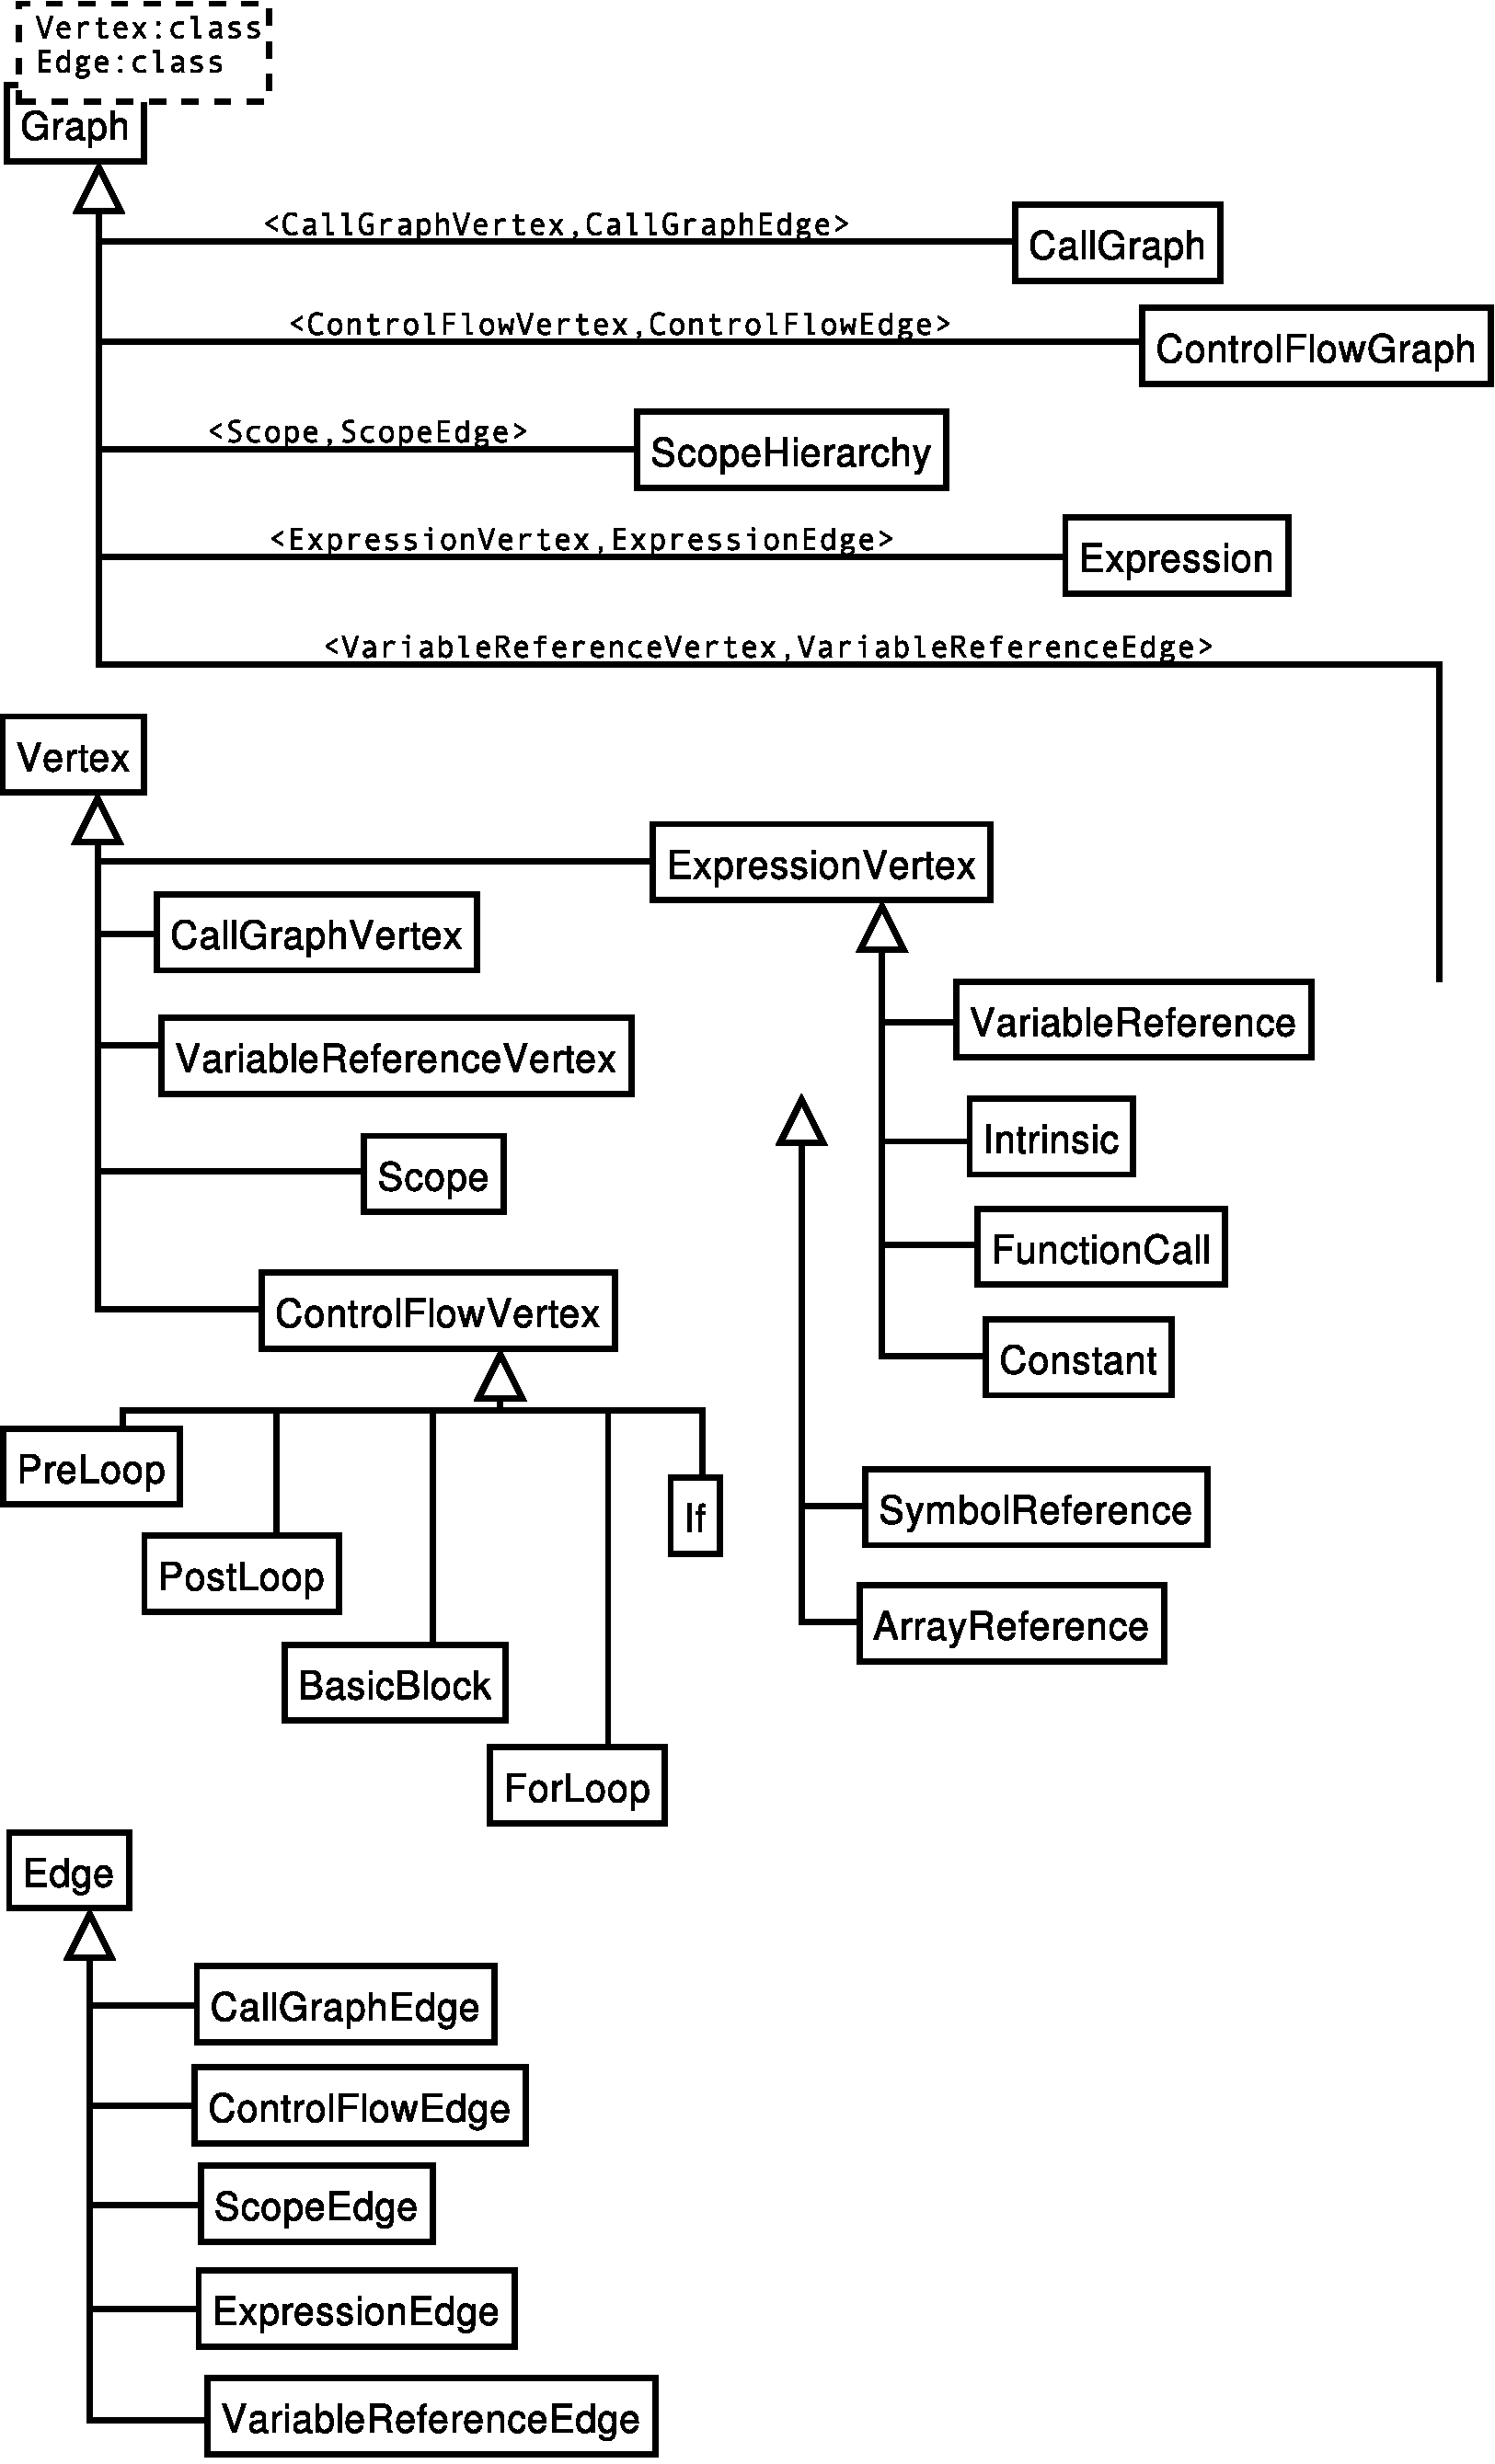
\includegraphics[width=.45\textwidth]{irInh}
  \caption{Simplified class inheritance in \xaifBooster} \label{fig:iri}
\end{figure}
The \xaifBooster\ data structure  
closely resembles the information one would find in a 
compiler's high level internal representation. 
the boost graph library \cite{boostWeb}
and the Standard C++ Library\cite{libstdcWeb}.
\reffigBS{fig:iri} and \reffig{fig:irc} show simplified subsets of the classes 
occurring in the \xaifBooster\ data structure in the inheritance 
as well as the composition hierarchy.  
\begin{figure}[htb]
  \centering 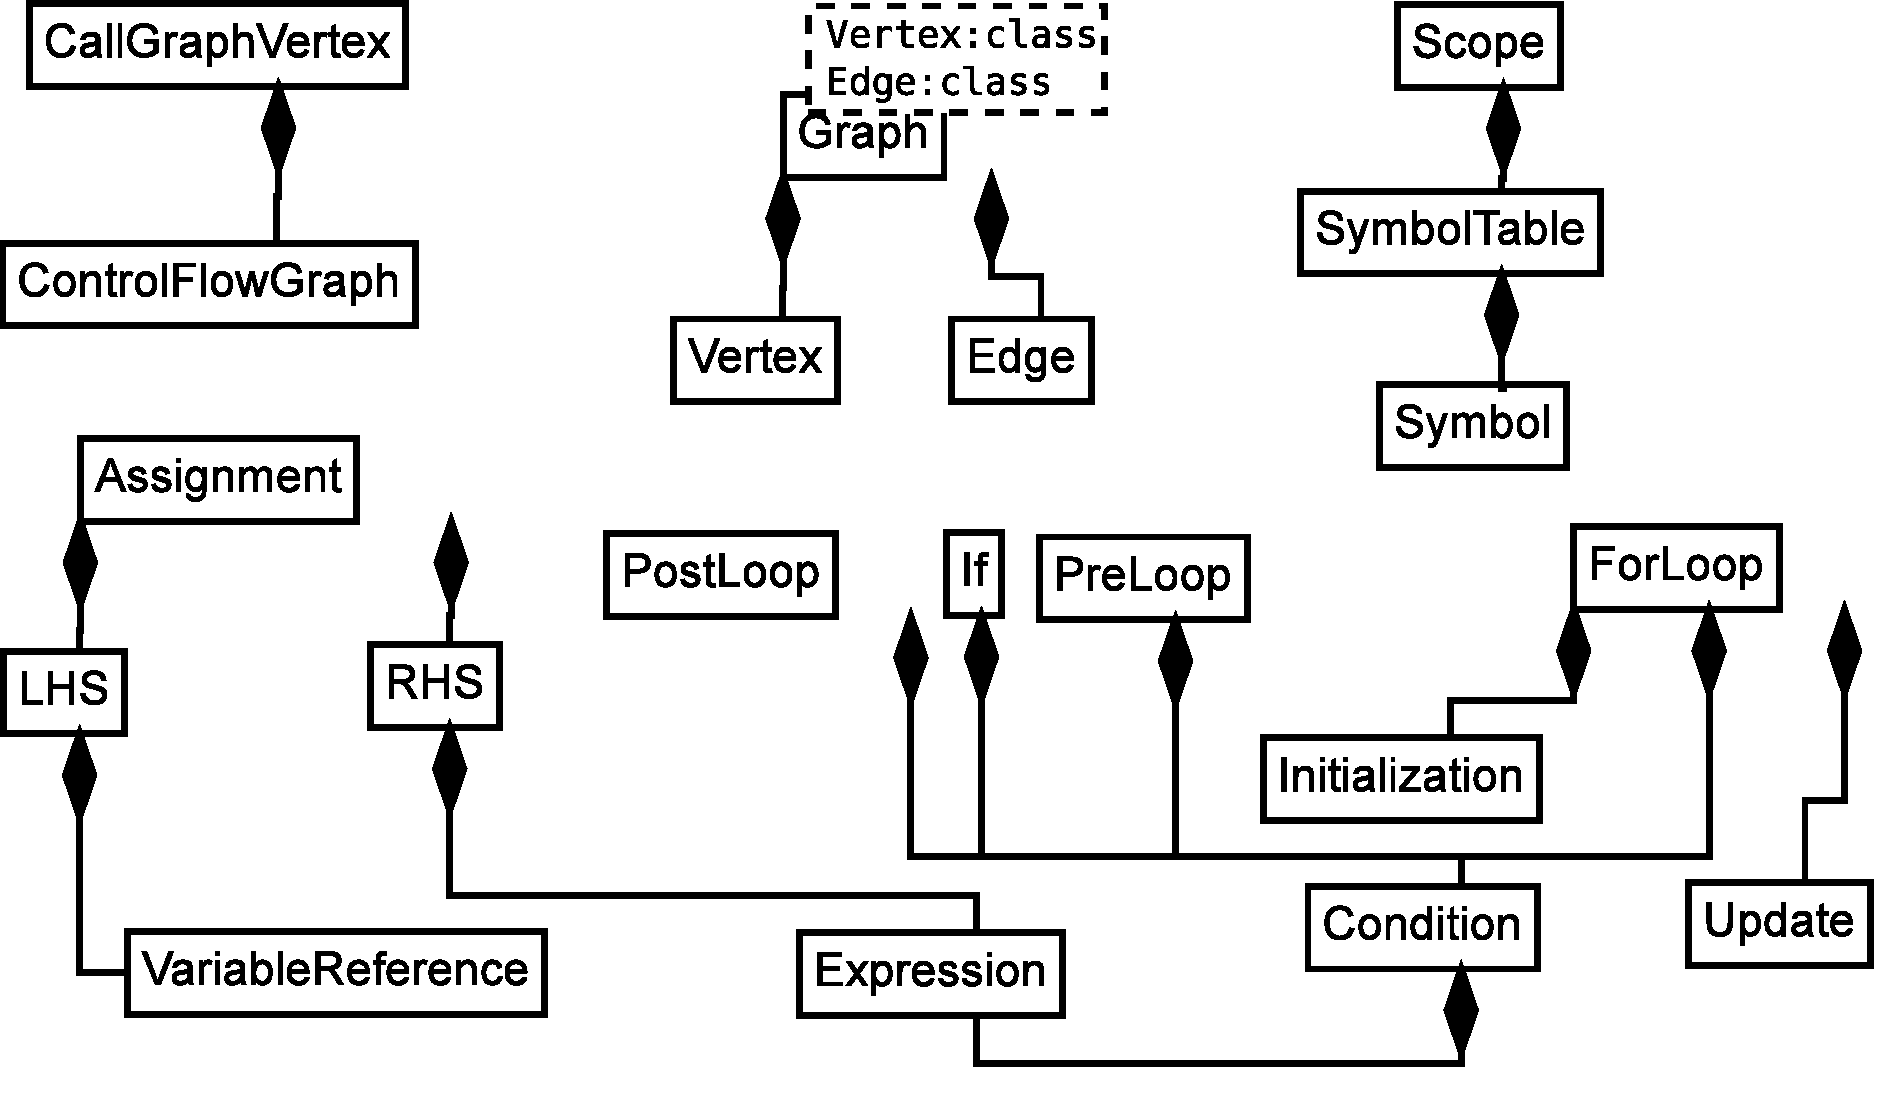
\includegraphics[width=.45\textwidth]{irComp}
  \caption{Simplified class composition in \xaifBooster} \label{fig:irc}
\end{figure}
A doxygen generated documentation of the entire data structure 
can be found on the \OpenAD\ website \cite{openadWeb}.
The class hierarchy is organized top down with 
a single \code{CallGraph} instance as the top element. 
The top down structure is also imposed on the ownership of dynamically 
allocated elements. 
Wherever possible, the class interfaces encapsulate dynamic 
allocation of members.  
Only in cases of containment of polymorphic elements is explicit dynamic allocation 
outside of the owning class' members appropriate. 
In these cases the container class interface naming and documentation 
indicates the assumption of ownership of 
the dynamically allocated elements being supplied to the container class. 
An example is the graph class \code{Expression} accepting vertex instances that can be 
\code{Constant}, \code{Intrinsic} , etc.

The transformation algorithms are modularized to enable reuse in different 
contexts. 
\begin{figure}
  \centering 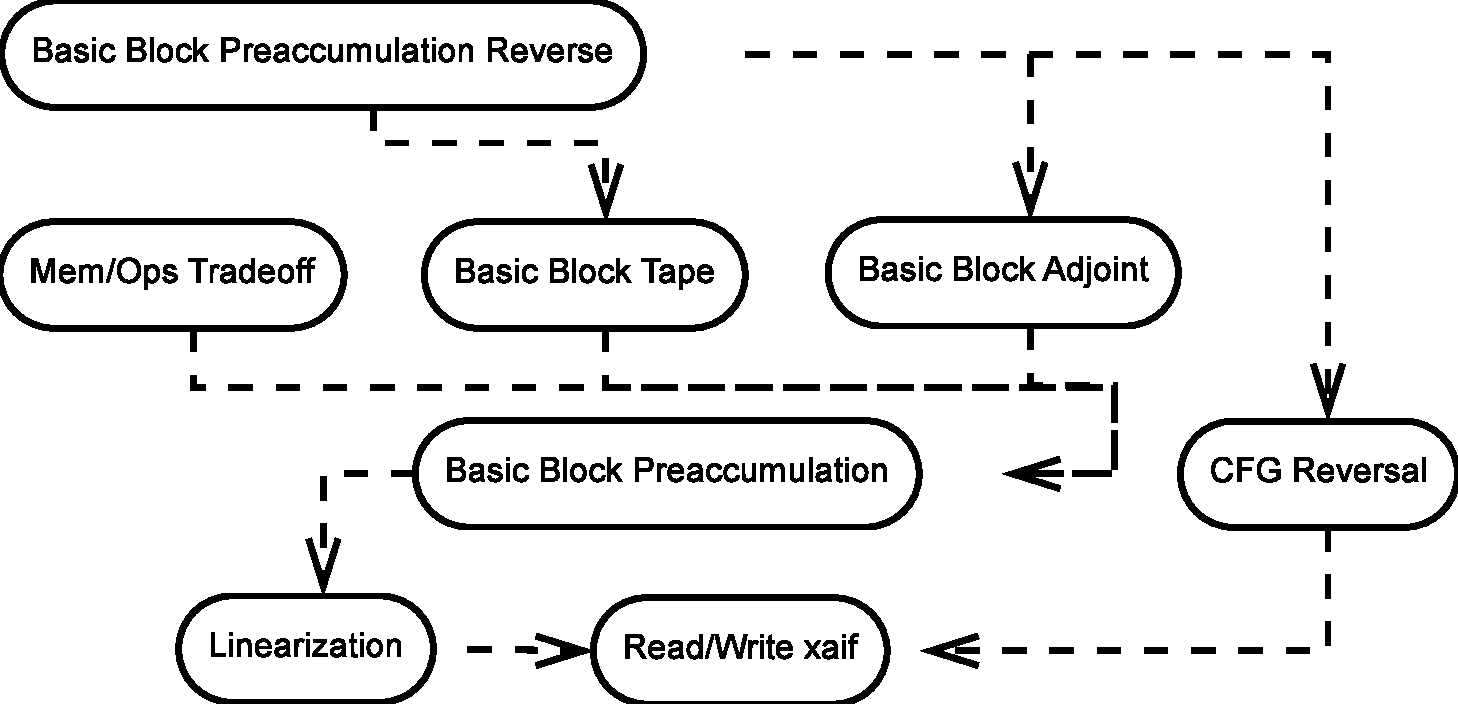
\includegraphics[width=.45\textwidth]{allAlgs}
  \caption{\xaifBooster\ algorithms} \label{fig:allAlgs}
\end{figure}
\reffig{fig:allAlgs} shows some implemented algorithms with dependencies.
To avoid conflicts the transformation algorithms the data structure representing the input code  
is never directly modified. 
Instead, any data representing modifications or augmentations of the 
original representation element in a class \code{<name>}
are held in algorithm specific instances of class \code{<name>Alg}.
The association is done via mutual references accessible 
through \code{get<name>AlgBase()} and \code{getContaining<name>()} respectively.
The instantiation of the algorithm specific classes follows 
the factory design pattern. The factory instances in turn are controlled 
by a transformation algorithm specific \code{AlgFactoryManager} classes. 
Further details can be found in \cite{UtNa03STI}, however, the code 
code for this mechanism is fairly self-explanatory.  

In the following sections we want to concentrate on the transformation 
the algorithms execute while deferring to the generated code 
documentation for most technical details.

Each algorithm has a driver \code{t.pp} (compiled into a binary \code{t}) 
found in \code{algorithms/<the\_algorithm\_name>/test/} 
that encapsulates the algorithm 
in a stand-alone binary which provides the functionality described 
in the following 
sections. For details on the invocation and command line options refer to 
\refsec{sec:manualPipeline}.

% -----------------------------------------------------------------------------------------
\subsubsection{Reading and Writing \xaif}\label{ssssec:readWriteXaif}
Reading and Writing the \xaif\ is part of basic infrastructure
found in the sources in \code{system/}.
Parsing is done through the Xerces C++ XML parser \cite{xercesWeb}
such that the XML element handler implementations, see \code{system/src/XAIFBaseParserHandlers.cpp},
build the \xaifBooster\ data 
structure from the top down. 
As an additional consistency check all components that read \xaif\ data 
have the validation according to the schema enabled. Beyond the schema 
validation these components perform validity checks. Therefore, 
manual modifications of \xaif\ data , while possible, should 
be done judiciously. 

The unparsing of the transformed data structure into \xaif\ is performed 
through a series of that traverses the data structure and the 
respective algorithm specific data. 
For information of the files containing the \xaif\ representation refer to 
\refsec{sec:manualPipeline}.

Aside from the parsing of the actual input \xaif\ there is also the so called 
{\em 
  catalog of inlinable intrinsics
} 
supplied as an XML following a specialized schema in \xaif, see  
\refsec{sssec:linearization} and \refsec{sssec:wtxxtw}.
There is also a driver at this level found in \code{system/test/t.cpp} used 
to verify reading and writing functionality. It can be used to establish 
that the tool pipeline preserves the semantics of the original program when 
no transformation is involved. 

% -----------------------------------------------------------------------------------------
\subsubsection{Linearization}\label{sssec:linearization}

\refsec{chap:ADIntro} explained the computation of 
the local partial derivatives $c_{ji}$ that can be thought of as edge labels 
in the computational graph $G$. 
Per canonicalization (see \refsec{sssec:Canonicalization}) 
all elemental $\phi$ 
occur only in the right-hand side of an assignment. 
For each $\phi$ we look up the definition of the respective partials in 
the intrinsics catalog. 
{\color{red} [ not sure  how much detail is necessary ] } 
The partials are defined in terms of positional arguments, see 
\reffig{fig:divExample}. 
\begin{figure}
  \centering 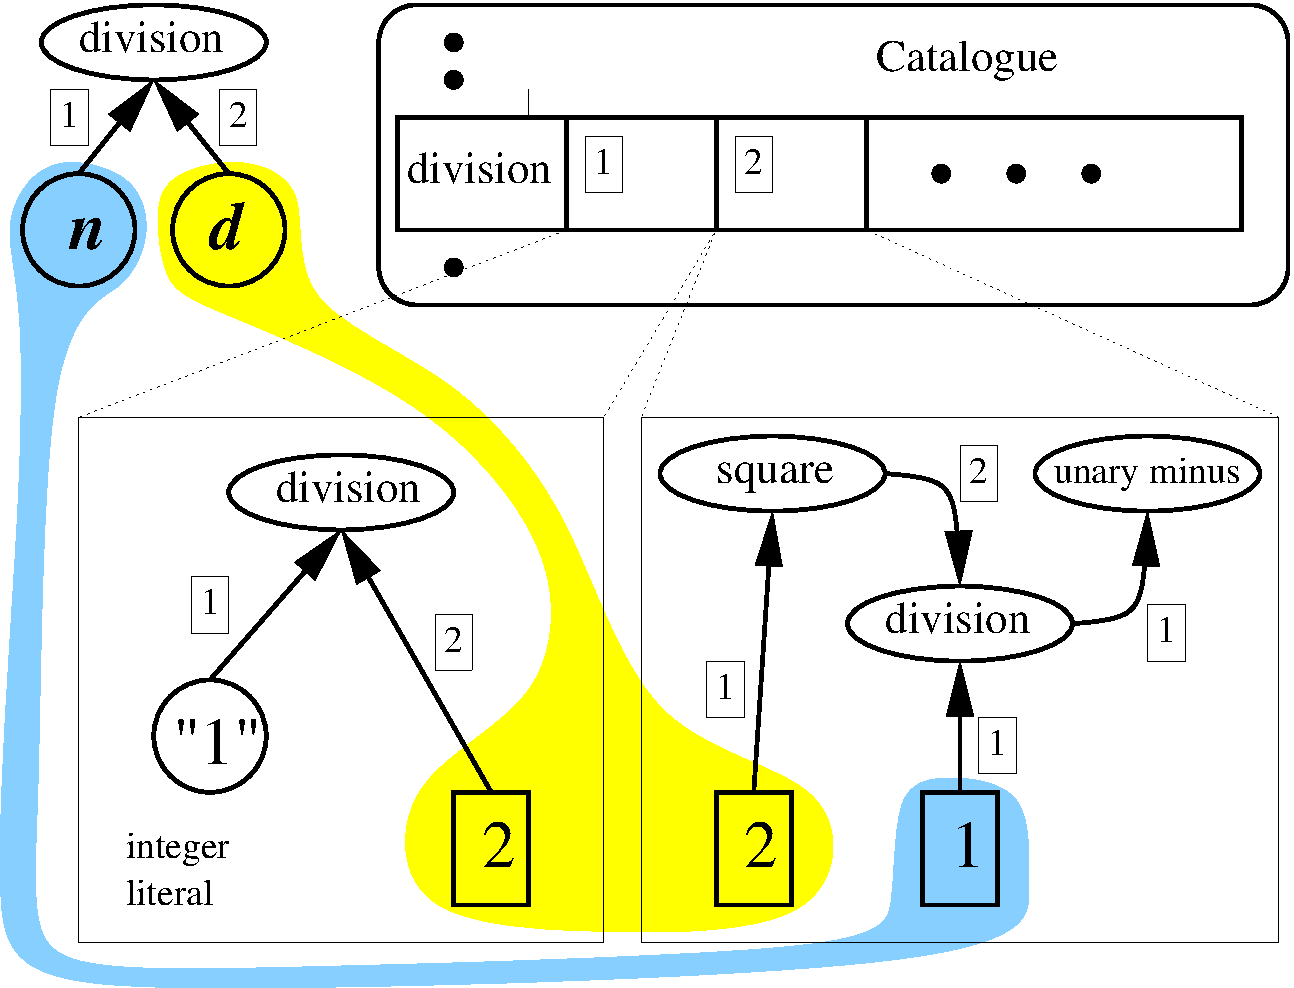
\includegraphics[width=5cm]{divIntrinsic}
  \caption{Partial expressions for the division operator} \label{fig:divExample}
\end{figure}

Because of this, 
the right-hand-side expression may have to be split up into 
subexpressions to assign intermediate values to ancillary variables 
that can be referenced in the partial computation, for an example see 
the code shown in \reffig{fig:toyAndPartials}.  
In cases of the left-hand-side variable occurring on the right-hand-side 
(or being may-aliased to a right-hand-side variable, 
see \refsec{ssec:openanalysis}) we also require an extra assignment to 
delay the (potential) overwrite until after the partials depending on 
the original variable value have been computed.
The result of the Linearization is a representation for 
code containing the potentially split 
assignments along with assignments for each non-zero edge label $c_{ji}$.
These representations are contained in the \code{xaifBoosterLinearization::AssignmentAlg} instances associated with each assignment in the \xaif.
The generated code after unparsing to Fortran 
is compilable but does by itself not compute useful 
derivative information at the level for the target function $\bmf$. The 
transformation driver is 
used to verify the results of the linearization transformation.

% -----------------------------------------------------------------------------------------
\subsubsection{Basic Block Preaccumulation}\label{sssec:BBPreacc}

This transformation generates a code representation that can be used 
to compute derivatives in forward mode. It builds upon the Linearization
done in \refsec{sssec:linearization}. 
The first step constructs the 
computational graphs $G$ 
for contiguous 
assignment sequences in a given \basicblock. To ensure semantic 
correctness of the graph being constructed in the presence of 
aliasing it relies on alias analysis and define-use/use-define chains 
supplied by \OpenAnalysis, see \refsec{ssec:openanalysis}.
The algorithm itself is described in detail in \cite{Utk04FBB}.
Because the analysis results supplied by \OpenAnalysis\ are always 
conservatively correct it may not be possible to flatten all 
assignments into a single computational graph. In such cases 
a sequence of graphs is created. Likewise, the occurrence 
of a subroutine call leads to a split in the graph construction. 
In the context of \refsec{chap:ADIntro} one may think of the sets of 
assignments forming each of these graphs as a separate \basicblock. 
The driver for the algorithm allows to disable 
the graph construction across assignments and restrict it to 
single right-hand sides by adding the \code{-S} command 
line flag. 

Based on the constructed $G$ an elimination sequence has to be determined.
To allow a choice for the computation of the elimination sequence 
the code uses the interface coded in \code{algorithms/CrossCountryInterface/}
and by default calls the \angel\ library \cite{angelWeb,AGN03,SAGA}.
\angel\ determines an elimination sequence and returns it as 
fused multiply add expressions in terms of the edge references.
There are several heuristics implemented within \angel\ that control 
the selection of elimination steps and thereby the preaccumulation code 
that is generated.  The algorithm code calls a default set of heuristics. 
However, all heuristics use the \code{CrossCountryInterface} and therefore 
different heuristics can be selected with minimal changes in algorithm code.   

The second step in this transformation is the generation of 
preaccumulation code. 
First it  turns the abstract expression graphs returned by \angel\ 
into assignments and resolves the edge references into 
the  labels $c_{ji}$. The resulting code resembles what 
we show in  \reffig{fig:toyAccumulation}. 
Then it generates the code that eventually performs the \saxpy\ 
operations shown in \refeqn{eqn:bbfm}. 
Considering the input and output variables $\bmx_j$ and $\bmy_j$ of a \basicblock\ the code generation 
also ensures proper propagation of $\dot{x}_i^j$ of variables $ x_i^j \in  \bmx_j \cap \bmy_j$ 
by saving the $\dot{x}_i^j$ in temporaries. The example in \reffig{fig:toyPreacc} illustrates this case. 
The detection of the intersection elements relies on the alias analysis provided by 
\OpenAnalysis.
To reduce overhead 
the generated \saxpy\ operations we generate \saxpy\ calls following the 
interface specified in \code{algorithms/DerivativePropagator/} for the following four cases:
\begin{equation}\label{eqn:fourSaxpy}  
  \mbox{(a):}\;\;\dot{y} = \frac{\partial y }{\partial x }\cdot \dot{x},\; 
  \mbox{(b):}\;\;\dot{y} = \frac{\partial y }{\partial x }\cdot \dot{x} + \dot{y},\; 
  \mbox{(c):}\;\;\dot{y} = \dot{x},\;
  \mbox{(d):}\;\;\dot{y} = 0\quad .
\end{equation}	
The generated code is executable and represents an overall forward mode 
according to \refeqn{eqn:bbfm} with \basicblock\-local preaccumulation in 
cross-country fashion. 

% -----------------------------------------------------------------------------------------
\subsubsection{Memory/Operations Tradeoff}\label{sssec:MMTradeOff}

This algorithm can be seen as an alternative to the \angel\ library. 
Like \angel\ it uses the \code{CrossCountryInterface}. In its implementation 
it replaces the call to \angel\ with one to its own internal routines that
determine an elimination sequence according to a selectable set of heuristics. 
In difference to the \angel\ heuristics  they 
aim for a tradeoff between the number of operations required to complete an elimination 
sequence on the one hand and the temporal locality of the $c_{ji}$ in memory on the other hand. 
The rationale for these heuristics is the observation that in many modern 
computer architectures the performance is memory bound, i.e. a few additional 
operations can easily be absorbed if we keep all the necessary data in cache. 
All heuristics take as an input a set $\Theta \neq \emptyset $ of target elements, that is 
a set of vertices or edges from $G$, or faces from $\cal G$. 
The heuristic selects a nonempty subset $\Theta'\subseteq \Theta $ from this set. 
In order to determine a single elimination target a sequence of heuristics may be applied 
that successively shrink the target set concluding with a tie breaker such as 
selecting the next target that would be eliminated in forward or reverse mode. 
\reftab{tab:memOpsHeur} describes the selection criterion of a heuristics with 
respect to an elimination technique.  If the selection criterion is not met 
by any target in $\Theta$, then $\Theta'=\Theta$. 
\begin{table}[htb]
  \begin{tabular}{|l|c|c|c|}\hline
    & \code{VERTEX} & \code{EDGE} & \code{FACE} 
    \\\hline %---------------------------------------
    \code{SIBLING} 
    &
    \begin{minipage}{.4\linewidth}
      \footnotesize
      select vertices that share at least one predecessor
      and successor with the most recently eliminated vertex.
    \end{minipage}
    & N/A & N/A
    \\\hline %---------------------------------------
    \code{SIBLING2} 
    &
    \begin{minipage}{.4\linewidth}
      \footnotesize
      select vertices with the maximal product of 
      the number of predecessors and the number of 
      successors shared with the most recently eliminated vertex
    \end{minipage}
    &
    \begin{minipage}{.2\linewidth}
      \footnotesize
      select edges with the same source / target and the 
      maximal number of successors / predecessors shared with the 
      successors / predecessors of 
      the most recently front / back eliminated edge
    \end{minipage}
    & N/A 
    \\\hline  %---------------------------------------
    \code{SUCCPRED} 
    &
    \begin{minipage}{.4\linewidth}
      \footnotesize
      select vertices  that were either predecessors or successors of
      the most recently eliminated vertex
    \end{minipage}
    & N/A & N/A 
    \\\hline %---------------------------------------
    \code{ABSORB} 
    & N/A & N /A &
    \begin{minipage}{.2\linewidth}
      select faces that are absorbed
    \end{minipage}
    \\\hline %---------------------------------------
    \code{MARKOWITZ} 
    &
    \begin{minipage}{.4\linewidth}
      \footnotesize
      select vertices with  the lowest Markowitz degree
    \end{minipage}
    &
    \begin{minipage}{.2\linewidth}
      \footnotesize
      select edges with the lowest Markowitz degree
    \end{minipage}
    &
    N/A
    \\\hline %---------------------------------------
    \code{FORWARD} 
    &\multicolumn{3}{c|}{
      select the target next in forward mode
    }
    \\\hline %---------------------------------------
    \code{REVERSE} 
    &\multicolumn{3}{c|}{
      select the target next in reverse mode
    }
    \\\hline %---------------------------------------
  \end{tabular}
  \caption{Heuristics selection criteria}\label{tab:memOpsHeur}
\end{table}
The driver allows a sequence of heuristics to be selected via string supplied as 
an argument to the commandline switch \code{-H}. The string needs to contain 
the target selection, one of \code{Vertex}, \code{EDGE}, or \code{FACE} followed by 
a sequence of heuristics that should include at least on of the tie breakers \code{FORWARD} or 
\code{REVERSE}. 
Obviously the data locality criteria still are rather simplistic but 
the code is easily extensible for more elaborate strategies. 

The generated code is executable and represents an overall forward mode 
according to \refeqn{eqn:bbfm} with \basicblock\-local preaccumulation in 
cross-country fashion. 

% -----------------------------------------------------------------------------------------
\subsubsection{Using the ANGEL Library}\label{sssec:angel}
{\color{red} [ JU: This was a placeholder to talk about the \angel\ lib 
  but I think I will remove this unless somebody strongly objects]}
% -----------------------------------------------------------------------------------------
\subsubsection{CFG Reversal}\label{sssec:cfgRevAlg}

\refsec{sec:cfReversal} explains the principal approach to the reversal 
of the CFG. The CFG reversal as implemented in this transformation is 
by itself not useful as unparsed code other than for checking the correctness without 
interference from other transformations. It is a major building block for 
the  
adjoint code generator described in \refsec{sssec:BBRev}. 
The \Loop\ counters and \branch\ identifiers are stored the same 
stack data structure that is used for the {\em tape} (introduced in 
\refsec{sec:cfReversal} and also used in \refsec{sssec:bbTA}.  
The reversal of loops and branches as detailed in \cite{NULF04CFR} assumes 
CFGs to be well-structured, that is, essentially to be free of arbitrary jump instructions 
such as \code{GOTO} or \code{CONTINUE}. 
It is of course possible to reverse such graphs, for instance by enumerating
all {\basicblock}s, recording the execution sequence and invoking them according 
to their recorded identifier in  large  \code {SWITCH} statement in reverse order.
Such a reversal is obviously less efficient than a code that, by employing proper 
control flow constructs, aids compiler optimization. 
For the same reason well tuned codes implementing the target function $\bmf$ will 
avoid arbitrary jumps and therefore we have not seen sufficient demand to implement 
a CFG reversal for arbitrary jumps. 

The reversal of  \Loop\ constructs such as \code{do i=1,10} replaces 
the loop variable \code{i} with a generated variable name, say \code{t} and we 
loop up to  the stored execution count which we will call  \code{c} here. 
Then the reversed \Loop\ is \code{do t=1,c}. Quite often the loop body contains 
array dereferences such as \code{a(i)} but \code{i} is no longer available in the 
reversed \Loop. We call this kind of \Loop\ reversal {\em anonymous}. 
To access the proper memory location \code{i} will have to be stored along with the 
\Loop\ counters and \branch\ identifiers in the tape stack.
To avoid this overhead the \Loop\ reversal may be declared {\em explicit}
by prepending \code{!\$openad xxx simple loop} to the \Loop\ in question. 
With this directive the original \Loop\ variable will be preserved,  
the reversed \Loop\ in our example constructed as \code{do i=10,1,-1} and 
no index values for the array references in the \Loop\ body are stored. 
In general the decision when an array index needs to be stored is better answered 
with a code analysis similar to TBR analysis \cite{HNP02}. 
Currently we do not have such  analysis available and instead 
as a compromise define the {\em simple}
\Loop\ which can reversed explicitly as follows. 
\begin{itemize}
  \parskip = -2pt
\item \Loop\ variables are not updated within the loop,
\item the \Loop\ condition does not use \code{.ne.},
\item the \Loop\ condition's left-hand side consists only of the \Loop\ variable,
\item the stride in the update expression is fixed,
\item the stride is the right-hand side of the top level \code{+} or \code{-} operator,
\item the loop body contains no index expression with variables that are modified within the loop body.
\end{itemize}
While these conditions can be relaxed in theory, in practice the effort to implement 
the transformation will rise sharply. Therefore they represent a workable compromise 
for the current implementation. 
Because often multidimensional arrays  are accessed with nested loops the 
\Loop\ directive when specified for the outermost loop will assume the validity 
of the above conditions for everything within the \Loop\ body including nested 
\Loop\ and \branch\ constructs. More details on this aspect can be found in 
\cite{UtLy05ERIF}. 
% -----------------------------------------------------------------------------------------
\subsubsection{Writing and Consuming the Tape}\label{sssec:bbTA}

\refsec{chap:ADIntro} explains the need to store the $\frac{\partial \phi_j}{\partial v_i}$ 
on the tape. 
The writing transformation\footnote{
  see {\tt algorithms/BasicBlockPreaccumulationTape/}
}
stores the nonzero elements of local
Jacobians $\bmJ_j$. It is implemented as an extension of the 
preaccumulation in \refsec{sssec:BBPreacc} but instead of using the Jacobian elements 
in the forward 
\saxpy\ operations as in \refeqn{eqn:bbfm} we store them 
on a stack as shown for the example code in \reffig{fig:toyPreacc}(a). 
The tape consuming transformation algorithm\footnote{ 
  see {\tt algorithms/BasicBlockPreaccumulationTapeAdjoint/}
} 
reinterprets
the \saxpy\ operations generated in \refsec{sssec:BBPreacc} 
according to \reftab{tab:saxpyAdj}.
\begin{table}
  \begin{center}
    \begin{tabular}{l|l}
      forward & adjoint\\\hline
      (a): $\dot{y} = \frac{\partial y }{\partial x }\cdot \dot{x}$           & $\overline{x} = \frac{\partial y }{\partial x }\cdot \overline{y} + \overline{x},\;\;\overline{y}=0$ \\
      (b): $\dot{y} = \frac{\partial y }{\partial x }\cdot \dot{x} + \dot{y}$ & $\overline{x} = \frac{\partial y }{\partial x }\cdot \overline{y} + \overline{x}$ \\
      (c): $\dot{y} = \dot{x}$ 					            & $\overline{x} = \overline{y},\;\;\overline{y}=0$\\
      (d): $\dot{y} = 0$ 						            & $\overline{y} = 0$ 
    \end{tabular}
  \end{center}
  \caption{\saxpy\ operations  from \refeqn{eqn:fourSaxpy} and their corresponding adjoints} \label{tab:saxpyAdj}
\end{table} 
The tape writing and consumption implemented in these transformations are 
by themselves not useful as unparsed code other than for checking the correctness without 
interference from other transformations. 
They are, however, major building blocks for the  
adjoint code generator described in \refsec{sssec:BBRev}.
% -----------------------------------------------------------------------------------------
\subsubsection{Basic Block Preaccumulation Reverse}\label{sssec:BBRev}

This transformation\footnote{
  see {\tt algorithms/BasicBlockPreaccumulationReverse}
}
represents the combination of the various transformation 
into a coherent representation that, unparsed into code and post-processed, compiles 
as an adjoint model. 
For the postprocessing steps refer to \refsec{sssec:PostProcessor}.
Additional functionality is the generation of code that is able write and 
read checkpoints at a subroutine level, see also \refsec{sec:cgReversal}. 
This part of the transformation relies heavily on the results of side-effect analysis, see 
\refsec{ssec:openanalysis} and the inlinable subroutine call mechanism of 
the postprocessor, see \refsec{sssec:inline}, to accomplish the checkpointing. 
The driver offers command line options
\begin{itemize}
\item to change subroutine argument intents 
  such that checkpointing can take place; while checkpointing will 
  generally be needed this option is useful 
  for certain application scenarios where the intent change can be avoided.
\item  to validate the \xaif\ input against the schema; the validation takes 
  considerable time for large \xaif\ files
\item to specify a list of subroutines 
  that have a wrappers which should be called in its place
\item to force the renaming of all non-external subroutines which may be necessary 
  for applications which expose only portions of the code to \OpenADF.
\end{itemize}

% -----------------------------------------------------------------------------------------
\section{Language Dependent Components (\OpenADFortTk)}\label{sec:fortfe}

For simplicity we consider all language dependent components part 
of the \OpenAD\ Fortran Tool Kit (\OpenADFortTk). The following 
sections provide details for the various subcomponents that 
are used in transformation pipeline in the following sequence.
\begin{enumerate}	
\item The {\em canonicalizer} converts  
  programming constructs into a canonical form described in \refsec{sssec:Canonicalization}. 

\item The compiler front-end \mfefninety\  parses
  Fortran and generates an intermediate representation (IR)
  in the \whirl\ format, see \refsec{sssec:mfef}

\item \whirlToxaif\ is a bridge component that
  \begin{itemize}
  \item drives the various program analyses (see \refsec{ssec:openanalysis}),
  \item translates the numerical core of the program and  
    the results of the program analyses from \whirl\ to \xaif.
  \end{itemize} see also \refsec{sssec:wtxxtw}

\item \xaifTowhirl\ is bridge component that translates the 
  differentiated numerical core represented in \xaif\ 
  into the \whirl\ format. see \refsec{sssec:wtxxtw}.

\item \whirlTof\ is the ``unparser'' that converts \whirl\ to
  Fortran, see \refsec{sec:fortfe}

\item The {\em postprocessor} is the  final part of the transformation that
  performs template expansion as well as inlining substitutions, see \refsec{sssec:PostProcessor}

\end{enumerate}

% -----------------------------------------------------------------------------------------
\subsection{Canonicalization}\label{sssec:Canonicalization}
In \refsec{ssec:xaif} we explain how the restriction to the numerical core 
contributes to the  language independence of the transformation
engine.
Still, even for a single programming language, the numerical 
core often exhibits a large variability in expressing semantically 
identical constructs. 
To streamline the transformation engine we reduce this variability by 
{\em canonicalizing} the numerical core. 
Because it is done automatically, the canonicalization does \emph{not} 
restrict the expressiveness of the input programs supplied by the user.
Rather it is a means to reduce the development effort of the transformation engine. 
In the following we describe the canonical form. The canonicalizer mechanism is written 
in Python. All sources can be found under \code{OpenADFortTk/tools/canonicalize/}.
\begin{Can} \label{can:funcToSub}
  All function calls  
  are canonicalized into subroutine calls, see \reftab{tab:funcToSubCall}.
  \begin{table}
    \begin{tabular}{cc}
      \begin{minipage}{.4\linewidth}
        \fontsize{8pt}{9pt}
        \verbatimfile{code/funcCall.f}
      \end{minipage}
      & 
      \begin{minipage}{.4\linewidth}
        \fontsize{8pt}{9pt}
        \verbatimfile{code/funcToSub.f}
      \end{minipage}
      \\
      (a) & (b)
    \end{tabular}
    \caption{Canonicalizing a function(a) to a subroutine(b) call } \label{tab:funcToSubCall}
  \end{table}
  For the transformations, in particular the \basicblock\ level preaccumulation we 
  want to ensure that an assignment effects a single variable on the left-hand side. 
  Therefore  
  the right-hand-side expression ought to be side-effect free.
  While often not enforced by compilers, this is a syntactic requirement for Fortran programs.
  Rather than determining which user-defined functions have side
  effects, we pragmatically hoist \emph{all} user-defined functions.
  Consequently the right-hand-side expression of an assignment consists only of 
  elemental operations $\phi$ typically 
  defined in a programming language as built-in operators and intrinsics.
  The canonicalizer also performs the accompanying transformation of the function definition 
  \reftab{tab:funcToSub}(a) 	
  into a subroutine definition \reftab{tab:funcToSub}(b).  
  \begin{table}
    \begin{tabular}{cc}
      \begin{minipage}{.45\textwidth}
        \fontsize{8pt}{9pt}
        \verbatimfile{code/funcDef.f}	
      \end{minipage}
      & 
      \begin{minipage}{.4\textwidth}
        \fontsize{8pt}{9pt}
        \verbatimfile{code/subDef.f}	
      \end{minipage}
      \\
      (a) & (b)
    \end{tabular}
    \caption{Canonicalizing a function(a) to a subroutine(b) definition} \label{tab:funcToSub}
  \end{table}
  The \code{oad\_s\_} prefix can be adjusted by modifying \code{\_\_call\_prefix} in 
  \code{Lib/canon.py}. 
  A particular canonicalization of calls without canonicalization of definitions  
  is applied to the \code{max} and \code{min} intrinsics because in Fortran 
  they do not have closed form expressions for the partials. \OpenADF\ provides a run time 
  library containing definitions for the respective subroutines called instead.  
\end{Can}
\begin{Can}\label{can:param}
  Non-variable actual parameters are hoisted to temporaries.
  Any value passed to a routine could conceivably need augmentation. Furthermore, only variables
  can be augmented. 
  Consequently, {\OpenAD} hoists all non-variable actual parameters into temporaries.
  \begin{table}
    \begin{center}
      \begin{tabular}{cc}
        \begin{minipage}{.3\linewidth}
          \code{call foo(x*y)}
        \end{minipage}
        & 
        \begin{minipage}{.3\textwidth}
          \fontsize{8pt}{9pt}
          \verbatimfile{code/hoist.f}	
        \end{minipage}
        \\
        (a) & (b)
      \end{tabular}
    \end{center}
    \caption{Before(a) and after(b) hoisting a non-variable parameter}\label{tab:hoistingParameters}
  \end{table} 
\end{Can}
In the Fortran context there is also the need to canonicalize certain constructs 
to support the implementation with a specific active type. 
\begin{Can}\label{can:comBlock}
  Common blocks are converted to modules.
  The purpose of this canonicalization is to ensure proper initialization of 
  active global variables.
  The method of conversion is to simply declare the elements of the common block as module variables. 
  Care must be taken to privatize and declare any symbolic size parameters
  for elements of the common block. See \reftab{tab:cbToM} for an example.
  \begin{table}
    \begin{center}
      \begin{tabular}{cc}
        \begin{minipage}{.3\linewidth}
          \fontsize{8pt}{9pt}
          \verbatimfile{code/commonBlock.f}	
        \end{minipage}
        & 
        \begin{minipage}{.3\textwidth}
          \fontsize{8pt}{9pt}
          \verbatimfile{code/cbModule.f}	
        \end{minipage}
        \\
        (a) & (b)
      \end{tabular}
    \end{center}
    \caption{Converting a common block (a) to a  module (b)}\label{tab:cbToM}
  \end{table}
\end{Can}
Because none of the above canonicalizations are intended to produce manually 
maintainable code we prefer simplicity over more sophisticated transformations 
e.g. a module generator which abstracts dimension information shared between common blocks. 

% -----------------------------------------------------------------------------------------
\subsection{Compiler Front-End Components (from \OpenSixtyFour)} \label{sssec:mfef}

The choice of \OpenSixtyFour\ for some of the programming-language-dependent 
components ensures some initial robustness of the tool that is afforded by an 
industrial-strength compiler. 
The Center for High Performance Software Research (HiPerSoft) at Rice University 
develops \OpenSixtyFour\ \cite{open64Web} as a 
multi-platform version of the SGI Pro64/Open64 compiler
suite, originally based on SGI's commercial MIPSPro compiler.

\OpenADF\ uses the parser, an internal representation and the unparser 
of the \OpenSixtyFour\ project.
The classical compiler parser \mfefninety\ produces a representation of the Fortran 
input in a format known as very high level or source level \whirl\ . 
The \whirl\ representation can unparsed into Fortran using the 
tool \whirlTof.
The source level \whirl\
representation resembles a typical abstract syntax tree with the 
addition of machine type deductions. 
The original design of \whirl\ in particular the descent to 
lower levels closer to machine code  enables good optimization 
for high performance
computing in Fortran, C, and C++. HiPerSoft's main
contribution to the \OpenSixtyFour\ community has been the source 
level extension to \whirl\
which is geared towards supporting source-to-source transformations and 
it 
has invested significant effort in the \whirlTof\ unparser.

For the purpose of AD, user-supplied hints and required 
input is typically not directly
representable in programming languages such as Fortran.  
For example,
an AD tool must know which variables in the code for $\bmf$ are
independent and which are dependent. 
While it is possible to supply this information externally, 
for instance with a configuration file, we introduced a special
pragma facility, encoded within Fortran comments. 
While pragmas are intrusive they have the added advantage to be 
parsed by the front-end and be associated with a given context in the code.
Thereby code and AD information is easier kept in sync.  
For \OpenADF\ we extended the
\OpenSixtyFour\ components to generate and unparse these pragma nodes represented in \whirl.
The behavior is 
similar to many other special-purpose Fortran pragma systems such as
OpenMP \cite{openmpWeb}. 
To specify a variable
$y$ as a dependent, the user writes \code{!\$openad dependent(y)},
where \code{\$openad} is the special prefix that identifies \OpenAD\
pragmas.   
To provide flexibility we introduced a generic
\code{!\$openad xxx <some text>} pragma\footnote{
  The mnemonic behind the name is that
  as $x$ is the typical variable name, so \code{!\$openad xxx} is the
  {\em variable} pragma.} 
that can communicate arbitrary pieces of
text through the pipeline. 
These generic pragmas can be associated with whole procedures, 
single statements, or groups
of statements. They provides an easy way 
to implement additional user hints while eliminating the significant
development costs associated with modifying \OpenSixtyFour.

% -----------------------------------------------------------------------------------------
\subsection{Translating between \whirl\ and \xaif}\label{sssec:wtxxtw}

\begin{figure}
  \scriptsize
  \verbatimfile{code/daerfj.f90}
  \caption{Example Fortran code}\label{fig:exampleFortranCode}
\end{figure}

\begin{figure}
  \scriptsize
  \verbatimfile{code/daerfj.whirl}
  \caption{Part of whirl for \reffig{fig:exampleFortranCode}}\label{fig:exampleWhirlCode}
\end{figure}

\begin{figure}
  \scriptsize
  \verbatimfile{code/daerfj.xaif}
  \caption{Part of \xaif\ for \reffig{fig:exampleFortranCode}}\label{fig:exampleXaifCode}
\end{figure}

The translation of \whirl\ into
\xaif\ (\whirlToxaif), feeding it to the transformation engine, and
then backtranslating the differentiated \xaif\ into \whirl\
(\xaifTowhirl) are crucial parts of the tool pipeline.  
Two distinguishing features of \xaif\ shape the
contours of \whirlToxaif\ and \xaifTowhirl.  

First, because \xaif\
represents only the numerical core of a program, many \whirl\
statements and expressions are not translated into \xaif\.  For
instance, \xaif\ does not represent dereferences for user-defined types 
because numerical operations simply will not involve the user defined 
type as such but instead always the numerical field that eventually is a member 
of the user defined type (hierarchy). 
Derived type references are therefore {\em scalarized}. This consists of converting
the derived type reference into a canonically named scalar variable.
To ensure correctness, this scalarization must be undone upon backtranslating 
to \whirl. The effect can be observed in the generated \xaif\ for \code{v\%f} where 
the dereference 
shows up for example 
as \code{<xaif:SymbolReference vertex\_id="1" scope\_id="4" symbol\_id="scalarizedref0"\/>}
and in the \xaif\ symbol table we would find \code{scalarizedref0} as a scalar variable with 
a type that matches that of \code{f}. 
However, variable references of user defined type can still show up in the \xaif\ for 
instance as subroutine parameters. Such references are listed with an 
{\em opaque} type. Statements in the original code that do not have an 
explicit representation in the  \xaif, 
such as I/O statements, take the form of annotated markers that retain 
their position in the representation during the transformation of the \xaif.  
Given the original
\whirl\ and the differentiated \xaif\ (with the scalarized objects, opaque types
and annotated markers intact), \xaifTowhirl\ is able generates new \whirl\ representing the
differentiated code while restoring the statements and types not shown in the \xaif.   

Second, \xaif\ provides a way to represent the results of  common
compiler analyses.  To provide these to the transformation engine 
\whirlToxaif\ acts as a driver for the analyses provided by the 
\OpenAnalysis\ package, see \refsec{ssec:openanalysis}.
In particular it implements the abstract \OpenAnalysis\ interface
to the \whirl\ IR. The results returned by \OpenAnalysis\ are then 
translated into a form consistent with \xaif.

The companion tool \xaifTowhirl\ backtranslates \xaif\ into \whirl. 
As indicated above it has to take care of restoring filtered out 
statements and type information. Because the differentiated \xaif\ 
relies on postprocessing, see \refsec{sssec:PostProcessor}, 
its other major challenge is the 
creation of \whirl\ that contains the postprocessor directives related to
three tasks to be accomplished by the postprocessor. 
\begin{itemize} 
\item The declaration and use of the active variables;
\item The placement of inlinable subroutine calls;
\item The demarcation of the various alternative subroutine bodies used in the subroutine template replacements.
\end{itemize}  

% -----------------------------------------------------------------------------------------
\subsection{Postprocessing}\label{sssec:PostProcessor}
The postprocessor performs the three tasks outlined at the end of \refsec{sssec:wtxxtw}.

\subsubsection{Use of the Active Type}\label{sssec:activeType}
The simplest postprocessing task is the concretization of the active variable declarations 
and uses. The main rationale for postponing the concretization of the active type is flexibility 
with respect to the actual active type implementation. The current postprocessor is 
written in Perl\footnote{ 
The source code can be found under {\tt OpenADFortTk/tools/multiprocess/}.
A rewrite in Python reusing the same Fortran parsing functionality of the canonicalizer is underway.
}
and therefore is much easier to adapt to a changing active type implementation than to 
find find the proper \whirl\ representation and modify \xaifTowhirl\ to create it.
However, it should be noted right away, that the ease of adaptation is clearly correlated to the 
simplicity and in particular the locality of the transformation. The advantage disappears with 
increased complexity of the transformation.   
For an active variable, for example  \code{v},  the representation created 
by \xaifTowhirl\ in \whirl\ and then unparsed to Fortran,
shows up as \code{TYPE (OpenADTy\_active) v}. 
In \whirl\ the type remains abstract because the accesses to the conceptual value and derivative components 
are represented as function calls \code{\_\_value\_\_(v)} and \code{\_\_deriv\_\_(v)} respectively.
The concretized versions created by the postprocessor for the current active type implementation, 
see \code{runTimeSupport/simple/OpenAD\_active.f90} are 
\code{type(active) v} for the declaration and simply \code{v\%v} for the value \code{v\%d} for 
the derivative component respectively and each subroutine will also receive an additional 
\code{USE} statement which makes the type definition in \code{OpenAD\_active} known. 

\subsubsection{Inlinable Subroutine Calls}\label{sssec:inline}
The second task, the expansion of inlinable subroutine calls, is more complex because 
any call expansion has now the scope of a subroutine body. The calls unparsed from \whirl\ to 
Fortran are regular subroutine call statements. They are however preceded by an inline  pragma
\code{!\$openad inline <name(parameters)>}  
that directs the postprocessor to expand the following call according to a definition 
found in an input file\footnote{
specified with command line option {\tt -i} which defaults to {\tt ad\_inline.f}
}, see also \code{runTimeSupport/simple/ad\_inline.f}.
For example, pushing a preaccumulated sub-Jacobian value as in  \reffig{fig:toyPreaccRev}(a) might appear 
in the code as\\
\hspace*{.05\textwidth}\begin{minipage}{.6\textwidth}
\fontsize{8pt}{9pt}
\verbatimfile{code/inlinePush.f}
\end{minipage}\\
for which we have a definition in \code{ad\_inline.f} as \\
\hspace*{.05\textwidth}\begin{minipage}{.6\textwidth}
\fontsize{8pt}{9pt}
\verbatimfile{code/inlinePushDef.f}
\end{minipage}\\
The postprocessor ignores the \code{DECLS} section and  expands this to\\
\hspace*{.05\textwidth}\begin{minipage}{.6\textwidth}
\fontsize{8pt}{9pt}
\verbatimfile{code/inlinePushExpanded.f}
\end{minipage}\\
%For example, using a preaccumulated sub-Jacobian value in a \saxpy\  as in  \reffig{what} might appear 
%in the code as
%\verbatimfile{code/inlineSaxpy.f}
%for which we have a definition in \code{ad\_inline.f} as 
%\verbatimfile{code/inlineSaxpyDef.f}
%and the postprocessor expands this to
%\verbatimfile{code/inlineSaxpyExpanded.f}
Note, that for flexibility 
any calls with inline directives for which the postprocessor cannot find an inline definition remain 
unchanged. For example we may instead compile the above definition for \code{Push} and link 
it instead.

\subsubsection{Subroutine Templates}\label{sssec:templates}
The third task, the subroutine template expansion is somewhat related the inlining. 
In our example above, the tape storage referred to in the \code{Push} need to be 
defined and in the design the subroutine template is the intended place for these definitions, 
in our example achieved through including the \code{use} statement in the template code, 
see \reffig{fig:jointACTemplate}.
The main purpose of the subroutine template expansion however is to orchestrate the 
call graph reversal. The reversal schemes introduced in \refsec{sec:cgReversal}
can be realized by carrying state through the call tree. 

The basic building blocks from the transformations in \refsec{sssec:xaifBooster}
are variants \code{S}$_i$ of the body of an original subroutine body \code{S}$_0$, 
each accomplishing one of the tasks shown as one of the squares with arrows in \reftab{tab:leg}. 
For instance, the taping variant is created by the transformation in \refsec{sssec:bbTA} or
the checkpointing by the transformation in \refsec{sssec:BBRev}. 
To integrate the $S_i$ 
into a particular reversal scheme, we need to be able to make all subroutine calls 
in the same fashion as in the original code and, at the same time, 
control which task each subroutine call accomplishes.  
We replace the original subroutine body with a branch structure in which each branch contains 
one $S_i$. 
The execution of each branch is determined by a global control structure whose members 
represent the state of execution in the reversal scheme.
The branches contain code for pre- and post-state transitions enclosing the respective $S_i$.
This ensures that the transformations producing the $S_i$
do not depend on any particular reversal scheme.
\begin{figure}
\hspace*{8ex}\begin{tabular}{l@{\hspace{.3cm}}c@{\hspace{1cm}}l@{\hspace{.3cm}}c}
(a)&
\begin{minipage}[t]{3cm}
\vspace*{-.3cm}
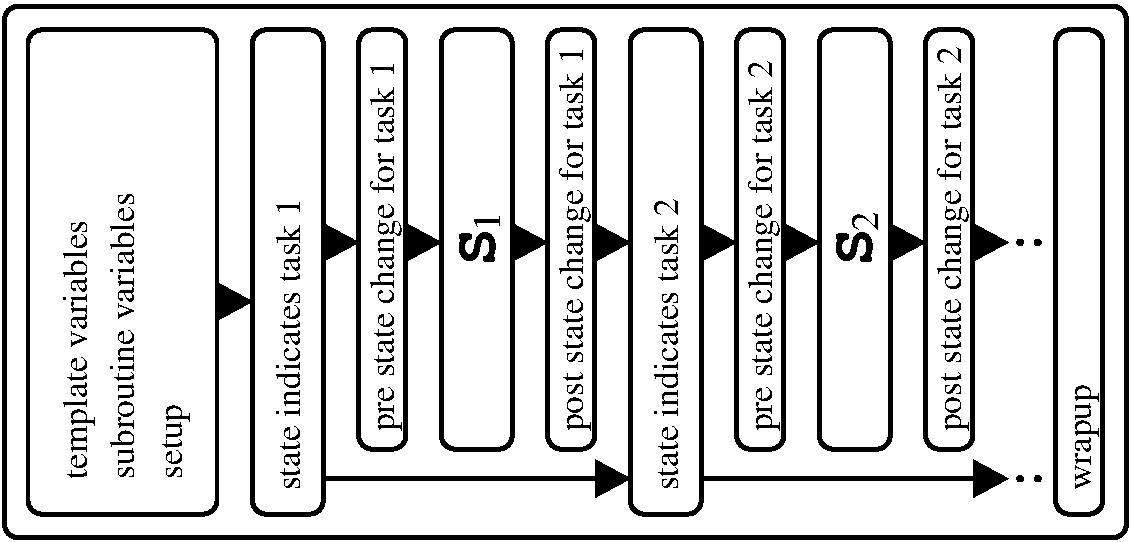
\includegraphics[height=3cm,angle=-90,origin=c]{code_template}
\end{minipage}&
(b)& 
\begin{minipage}[t]{4cm}
\fontsize{8pt}{9pt}
\verbatimfile{code/splitTemplate.pf}
\end{minipage}
\\
\end{tabular}
\caption{Subroutine template components (a), split-mode Fortran90 template (b) } \label{fig:codeTemplate}
\end{figure}
The postprocessor
inserts the \code{S}$_i$ into a subroutine template, schematically 
shown in \reffig{fig:codeTemplate}(a).
The template is written in Fortran. Each subroutine in the 
postprocessor Fortran input is transformed according to either 
a default subroutine template found in a \code{ad\_template.f} file or 
in a file specified in a \code{!\$openad XXX Template <file name>}
pragma to be located in the subroutine body. 
The input Fortran also contains \code{!\$openad begin replacement <}$i$\code{>} paired 
with pragmas \code{!\$openad end replacement}. Each such pair delimits a code variant \code{S}$_i$ 
and the postprocessor matched the respective identifier $i$ (an integer) with the 
identifier given in the template \code{PLACEHOLDER\_PRAGMA}.  

Split reversal is the simplest static call graph reversal. We first execute the entire computation 
with the augmented forward code $(S_2)$ and then 
follow with the adjoint $(S_3)$. 
From the task pattern 
shown in \reffig{fig:split} it is 
apparent that, aside from the top-level routine, there is 
no change to the state structure within the call tree.
Therefore, there is no need for state changes within the template. 
Since no checkpointing is needed either, we have only two tasks: 
producing the tape and the adjoint run.
\reffig{fig:codeTemplate}(b) shows a simple split-mode template, see also \code{runTimeSupport/simple/ad\_template.split.f}.
The state is contained in \code{rev\_mode}, a static Fortran90 variable, see \code{runTimeSupport/simple/OpenAD\_rev.f90}
of type \code{modeType} also defined in this module.  
In order to perform a split-mode reversal for the entire computation, a driver routine 
calls the top-level subroutine first in taping mode and then in adjoint mode.

\reffig{fig:joint} illustrates the task pattern for a joint reversal scheme that requires state changes 
in the template and requires more code alternatives. \reffig{fig:jointACTemplate} shows a 
simplified joint mode template, see also \code{runTimeSupport/simple/ad\_template.joint.f}. 
The state transitions in the template directly relate to the pattern 
shown in \reffig{fig:joint}. Each prestate change applies to the callees of the current 
subroutine. Since the argument store $(S_4)$ and restore $(S_6)$ do not contain any subroutine calls they 
do not need state changes. 
Looking at \reffig{fig:joint}, 
one realizes that the callees of 
any subroutine executed in plain forward mode $(S_1)$ 
never store the arguments (only callees of subroutines in 
taping mode do). 
This explains lines 18, 25, and 30. 
Furthermore, all callees of a routine currently in 
taping mode are not to be taped but instead run in plain forward mode, as reflected in lines 27 and 28. 
Joint mode in particular means that a subroutine called in taping mode $(S_2)$ has its adjoint $(S_3)$ executed immediately 
after $S_2$. 
This is facilitated by line 33, which makes the condition in line 35 true, and we execute 
$S_3$  without leaving the subroutine.  
Any subroutine executed in adjoint mode has its direct 
callees called in taping mode, which in turn triggers their respective adjoint run. This is done in 
lines 37--39.   
Finally, we have to account for sequence of callees in a subroutine; that is, when we are done with this subroutine, 
the next subroutine (in reverse order) needs to be adjoined. This process is triggered by calling the subroutine in taping mode, as done 
in lines 41--43. 
The respective top-level routine is called by the driver with the state structure having both {\tt tape} and 
{\tt adjoint} set to {\tt true}. 
\begin{figure}
\begin{center}
\vspace*{-1cm}
\begin{minipage}{.8\linewidth}
\fontsize{8pt}{9pt}
\verbatimfile{code/jointTemplate.pf}
\end{minipage}
\end{center}
\caption{Joint mode Fortran90 template with argument checkpointing} \label{fig:jointACTemplate}
\end{figure}
 
% #########################################################################################
\chapter{Tool Usage} \label{chap:Usage}
The following contains brief instructions how to obtain and use \OpenADF. 
While the principal approach will remain the same, future development may 
introduce slight changes. The reader is encouraged to refer to the 
up to date instructions on the \OpenADF\ website \cite{openadWeb}.

% -----------------------------------------------------------------------------------------
\section{Download and Build}\label{sec:dab}
All components are open source and readily available for download from 
the HiPerSoft CVS server at Rice University. Instructions to set up for anonymous 
CVS access are found at \url{http://hipersoft.cs.rice.edu/cvs/index.html#anonymous}.
The download is a 2 stage process where initially a skeleton repository is 
retrieved via \code{cvs co OpenAD}. This contains a few scripts and setup to 
retrieve and build all components. Then proceed as follows.
\begin{enumerate}
\item go into the \OpenADF\ download/build environment which was retrieved as described above:\\
\code {cd OpenAD}
\item retrieve all components from their various repositories by invoking\\
\code{./bin/goad}
\item set the environment for building and using \OpenADF\ for
\begin{itemize}
\item shell/ksh/bash etc users with\\
\code{source ./setenv.sh}
\item csh/tcsh etc. users with\\
\code{source ./setenv.csh}
\end{itemize}
\item We assume the GNU c/c++/f77 compilers versions 3.3.x to 3.4.4\footnote{
\OpenSixtyFour\ currently does not compile with gcc 4.x.
} 
and GNU make (gmake) to be in your \code{PATH}.
The complete set of all components can be build by invoking\\
\code{make}
\end{enumerate}
To update the sources to the latest version simply repeat the above steps 1 through 4 which 
executes CVS updates and performs a mostly incremental build.

% -----------------------------------------------------------------------------------------
\section{Code Prepaparation}

Pragma's etc. 

% -----------------------------------------------------------------------------------------
\section{Automatic Pipeline}
The components of \OpenADF\ transform the code in a predetermined sequence of steps, 
the {\em pipeline}. 
Depending on the particular problem there are certain variations to the pipeline 
that achieve a better performance of the generated code. 
The most common pipeline setups are encapsulated in a Perl script. 
The script is part of the skeleton environment that is used to download and build \OpenADF\  
and relies on the same environment setup.
Therefore user starts with steps 1 and 2 from \refsec{sec:dab}. 
The script is contained in the file
\code{OpenAD/tools/openad/openad}.
Invoking it with the \code{-h} option displays the 
script usage of which the mode choices are the most important.
\begin{description}
\item[\code{--bb-rev}] the default mode that produces adjoint code as explained in \refsec{sssec:BBRev},
\item[\code{--bb}] the tangent-linear mode as explained in \refsec{sssec:BBPreacc}, and
\item[\code{--memopstradeoff}] the tangent-linear mode with heuristics addressing data locality and operations count for the elimination sequence as explained in \refsec{sssec:MMTradeOff}.
\end{description}
As an example we use a code assumed to be in a file called head.f and transform this code 
by invoking \code{openad head.f}
which produces the adjoint version of \code{head.f} emitting the following messages.\\
\hspace*{.05\textwidth}\begin{minipage}{.6\textwidth}
\fontsize{8pt}{9pt}
\verbatimfile{code/openadScriptOutput.txt}
\end{minipage}\\
For larger projects it is obviously appropriate to customize the sequence 
by adding the steps outlined in \refsec{sec:manualPipeline} to a \code{Makefile}. 
 
% -----------------------------------------------------------------------------------------
\section{Manual Pipeline}\label{sec:manualPipeline}
The following illustrates the pipeline that could be implemented 
in a \code{Makefile} where we use successive file name postfixes to 
retain the transformation results at each stage.\\
\begin{longtable}{|@{\hspace{.5ex}}l@{\hspace{.5ex}}|l|l|}\hline
\scriptsize 1 & \multicolumn{2}{l|}{\scriptsize Canonicalization, see \refsec{sssec:Canonicalization}}\\\cline{2-3}
              & \scriptsize in (Fortran) & \scriptsize {\tt head.f}\\\cline{2-3}
              & \scriptsize out (Fortran) & \scriptsize {\tt head.canon.f} \\\cline{2-3}
              & \scriptsize command & \scriptsize {\tt python canon.v1.py head.f > head.canon.f}\\\cline{2-3}
              & \multicolumn{2}{l|}{
\begin{minipage}{.95\textwidth}
\scriptsize
The script is located at \\{\tt OpenADFortTk/tools/canonicalize/canon.v1.py}.
\end{minipage}
}\\\hline
\scriptsize 2 & \multicolumn{2}{l|}{\scriptsize Parsing, see \refsec{sssec:mfef}}\\\cline{2-3}
              & \scriptsize in (Fortran) & \scriptsize {\tt head.canon.f} \\\cline{2-3}
              & \scriptsize out (\whirl) & \scriptsize {\tt head.canon.B} \\\cline{2-3}
              & \scriptsize command & \scriptsize {\tt mfef90 -F -ffixed head.canon.f}\\\cline{2-3}
              & \multicolumn{2}{l|}{
\begin{minipage}{.95\textwidth}
\scriptsize
The binary is located at \\{\tt Open64/osprey1.0/targ\_ia32\_ia64\_linux/crayf90/sgi/mfef90}.\\
The {\tt -F} flag enables C preprocessing if needed, the {\tt -ffixed} indicates fixed format input.
\end{minipage}
}\\\hline
\scriptsize 3 & \multicolumn{2}{l|}{\scriptsize Translating to \xaif, see \refsec{sssec:wtxxtw}}\\\cline{2-3}
              & \scriptsize in (\whirl) & \scriptsize {\tt head.canon.B} \\\cline{2-3}
              & \scriptsize out (\xaif) & \scriptsize {\tt head.canon.xaif} \\\cline{2-3}
              & \scriptsize command & \scriptsize {\tt whirl2xaif -o head.canon.xaif head.canon.B}\\\cline{2-3}
              & \multicolumn{2}{l|}{
\begin{minipage}{.95\textwidth}
\scriptsize
The binary is located at \\{\tt OpenADFortTk/OpenADFortTk-i686-Linux/bin/whirl2xaif}.\\
The {\tt -o} flag allows to specify an output file, the default is {\tt stdout}.
\end{minipage}
}\\\hline
\scriptsize 4 & \multicolumn{2}{l|}{\scriptsize Transformation, see \refsec{sssec:xaifBooster}}\\\cline{2-3}
              & \scriptsize in (\xaif) & \scriptsize {\tt head.canon.xaif} \\\cline{2-3}
              & \scriptsize out (\xaif) & \scriptsize {\tt head.canon.xb.xaif} \\\cline{2-3}
              & \scriptsize command & \scriptsize {\tt <trans> -i head.canon.xaif -c <iCat> -o head.canon.xb.xaif}\\\cline{2-3}
              & \multicolumn{2}{l|}{
\begin{minipage}{.95\textwidth}
\scriptsize
The binary {\tt <trans>} is one of\\
{\tt xaifBooster/algorithms/BasicBlockPreaccumulation/test/t}, see \refsec{sssec:BBPreacc}\\
{\tt xaifBooster/algorithms/MemOpsTradeoffPreaccumulation/test/t}, see \refsec{sssec:MMTradeOff}\\
{\tt xaifBooster/algorithms/BasicBlockPreaccumulationReverse/test/t}, see \refsec{sssec:BBRev}\\
Each of the binaries prints a self explanatory usage message when invoked without any arguments. 
The intrinsics catalogue {\tt <iCat>} can be found in \\
{\tt xaif/schema/examples/inlinable\_intrinsics.xaif} 
\end{minipage}
}\\\hline
\scriptsize 5 & \multicolumn{2}{l|}{\scriptsize Translating to \whirl, see \refsec{sssec:wtxxtw}}\\\cline{2-3}
              & \scriptsize in (\whirl\ and \xaif) & \scriptsize {\tt head.canon.B  head.canon.xb.xaif} \\\cline{2-3}
              & \scriptsize out (\whirl) & \scriptsize {\tt head.canon.xb.x2w.B} \\\cline{2-3}
              & \scriptsize command & \scriptsize {\tt xaif2whirl head.canon.B head.canon.xb.xaif}\\\cline{2-3}
              & \multicolumn{2}{l|}{
\begin{minipage}{.95\textwidth}
\scriptsize
The binary is located at \\{\tt OpenADFortTk/OpenADFortTk-i686-Linux/bin/xaif2whirl}.\\
The optional {\tt --structured} flag indicates structured control flow, as required for 
the control flow reversal employed by the adjoint code transformation, see \refsec{sec:cfReversal}.
\end{minipage}
}\\\hline
\scriptsize 6 & \multicolumn{2}{l|}{\scriptsize Unparse to Fortran, see \refsec{sssec:mfef}}\\\cline{2-3}
              & \scriptsize in (\whirl) & \scriptsize {\tt head.canon.xb.x2w.B  head.canon.xb.xaif} \\\cline{2-3}
              & \scriptsize out (Fortran) & \scriptsize {\tt head.canon.xb.x2w.w2f.f} \\\cline{2-3}
              & \scriptsize command & \scriptsize {\tt whirl2f head.canon.xb.B}\\\cline{2-3}
              & \multicolumn{2}{l|}{
\begin{minipage}{.95\textwidth}
\scriptsize
The binary is located at \\{\tt Open64/osprey1.0/targ\_ia32\_ia64\_linux/whirl2f/whirl2f}.\\
It internally loads {\tt whirl2f\_be} located in the same directory.
\end{minipage}
}\\\hline
\scriptsize 7 & \multicolumn{2}{l|}{\scriptsize Postprocessing, see \refsec{sssec:PostProcessor}}\\\cline{2-3}
              & \scriptsize in (Fortran) & \scriptsize {\tt head.canon.xb.x2w.w2f.f}\\\cline{2-3}
              & \scriptsize out (Fortran) & \scriptsize {\tt head.canon.xb.x2w.w2f.pp.f} \\\cline{2-3}
              & \scriptsize command & \scriptsize {\tt perl multi-pp.pl head.f head.canon.xb.x2w.w2f.f}\\\cline{2-3}
              & \multicolumn{2}{l|}{
\begin{minipage}{.95\textwidth}
\scriptsize
The script is located at \\{\tt OpenADFortTk/tools/multi-process/multi-pp.pl}.\\
For tangent linear models the postprocessor requires the command line flag {\tt -f} while 
for inlining the default file name {\tt ad\_inline.f} can be changed with the {\tt -i} flag and for template expansion
the default template file name {\tt ad\_template.f} can be changed with the {\tt -t} flag. 
\end{minipage}
}\\\hline
\end{longtable}
The binaries used in steps 3, 5, and 6 all rely on the \code{libbe.so} \OpenSixtyFour\ backend library. 
It is located in \code{Open64/osprey1.0/targ\_ia32\_ia64\_linux/whirl2f/}.
 
% -----------------------------------------------------------------------------------------
\section{Compiling and Linking}\label{sec:compLink}
All Fortran produced by \code{whirl2f} needs definitions for \code{kind} 
variables that occur within the \code{whirl2f}-generated code. 
These definitions can be found in \code{runTimeSupport/all/w2f\_\_types.f90}.
The code produced by  transformation pipeline 
requires  implementations 
(\OpenADF\ supplies samples) for the following aspects.
\begin{itemize}
\item active type (see \code{runTimeSupport/simple/OpenAD\_active.f90})
\item checkpointing (only  for adjoint models, see \code{runTimeSupport/simple/OpenAD\_checkpoints.f90})  
\item taping (only  for adjoint models, see \code{runTimeSupport/simple/OpenAD\_tape.f90})  
\item state for call graph reversal (only  for adjoint models, see \code{runTimeSupport/simple/OpenAD\_rev.f90})
\end{itemize}
The compilation order for these various modules follows exactly the order given here.
The provided sample implementations work with the subroutine inlining and templates found in the same 
directory.

Finally, we need a {\em driver} that invokes the transformed routines and seeds and retrieves the derivatives.
Examples for such drivers can be found in \refsec{chap:application}.

% #########################################################################################
\chapter{Application}\label{chap:application}
This applications section intends to augment the explanations given so far. 
First we use a toy example to show how to embed the transformed code into 
a driver. The following sections illustrate practical concerns for real 
life applications. 
% -----------------------------------------------------------------------------------------
\section{Toy Example}\label{sec:toyExample}

Consider a toy example code  \reffig{fig:toyApp}(a) where we already inserted the 
dependent and independent declarartions, see \refsec{sssec:mfef}.
\begin{figure}
\begin{tabular}{cc}
\begin{minipage}{.4\textwidth}
\fontsize{8pt}{9pt}
\verbatimfile{code/appToy.f}
\end{minipage}
& 
\begin{minipage}{.4\textwidth}
\fontsize{8pt}{9pt}
\verbatimfile{code/appToyTlm.f}
\end{minipage}
\\
(a) & (b)
\end{tabular}
\caption{A toy example(a) and the modified signature for the tangent-linear model(b)}\label{fig:toyApp}
\end{figure}
Transformed into a tangent linear model \code{head} turns into a 
subroutine that has active parameters and the calling code, i.e. the driver, 
is written to seed (\code{x\%d}) and extract (\code{y\%d}) 
the derivatives according to \refeqn{eqn:JacVecProds}.
A very simple driver for the tangent-linear model is
\begin{figure}
\begin{tabular}{cc}
\begin{minipage}{.4\textwidth}
\fontsize{8pt}{9pt}
\verbatimfile{code/appToyDriver.f}
\end{minipage}
& 
\begin{minipage}{.4\textwidth}
\fontsize{8pt}{9pt}
\verbatimfile{code/appToyDriverOutput.txt}
\end{minipage}
\\
(a) & (b)
\end{tabular}
\caption{A toy example tangent-linear driver(a) and output(b)}\label{fig:toyAppDriver}
\end{figure}
Due to the simplicity of the example, the adjoint model version does not 
provide much insight other than the reversal of 
seeding (\code{y\%d}) and extraction (\code{x\%d})of the 
derivatives, see \reffig{fig:toyAppDriverAdj}.
\begin{figure}
\begin{tabular}{cc}
\begin{minipage}{.4\textwidth}
\fontsize{8pt}{9pt}
\verbatimfile{code/appToyDriverAdj.f}
\end{minipage}
& 
\begin{minipage}{.4\textwidth}
\fontsize{8pt}{9pt}
\verbatimfile{code/appToyDriverAdjOutput.txt}
\end{minipage}
\\
(a) & (b)
\end{tabular}
\caption{A toy example adjoint driver(a) and output(b)}\label{fig:toyAppDriverAdj}
\end{figure}

% -----------------------------------------------------------------------------------------
\section{Shallow Water Model}
In this section we will use a practical application to highlight 
advanced aspects arising for more complicated applications. 
The model is a time stepping scheme which eventually computes 
a scalar valued cost function. We generate an adjoint model 
to compute the gradient.  

% -----------------------------------------------------------------------------------------
\subsection{Collect and Prepare Source Files} 
The entire model consists of many subroutines distributed over various 
source files and the existing build sequence involves C preprocessing.
To perform the static code analysis as explained in \refsec{ssec:openanalysis}
all code that takes part in computation of the model has to be visible 
to the tool which means it has to be concatenated into a single file. 
It is possible to do this for all source files of the model but in many 
cases this will include code for ancillary tasks such as diagnostics 
and data processing not directly related to the model computation.
Often it is better to filter out such ancillary code. 
\begin{itemize}
\item The static code analysis and subsequently the code transformation
has to make conservative assumptions to ensure 
correctness, e.g. for alias analysis this means an overestimate of 
the memory locations that can alias each other. One of the effects of these potential aliases
are additional assignments in the generated code  which lead to 
a less efficient adjoint. Including ancillary sources may cause more conservative 
assumptions to be made and therefore lead to an unnecessary loss in efficiency.
\item While the numerical portions frequently have been tuned and made platform 
neutral the ancillary portions often are platform dependent and may contain
Fortran constructs that the language dependent components handle improperly or 
not at all. While all tools in principle strive for complete language coverage 
the limited development resources can often not be spared to cover 
infrequently used language aspects and rather need to be focused on features 
that actually benefit capabilities and efficiency for a wide range of applications.
\end{itemize}
As for all AD tools in existence today the above concerns also apply to 
\OpenADF\ and  users are kindly asked to keep them in mind when
preparing the source code.

\refsec{sec:toyExample} indicates the need for a modification 
to the code that drives the model computation to at least 
preform the seeding and extraction of the derivatives. 
The easiest approach to organize the driver is to identify (or create) 
a top level subroutine that computes the model with a single call. 
This routine and all code it requires to compute the model 
become the contents of the single file to be processed by the tool pipeline.
The independent and dependent variables should be identified in the top level routine.  

% -----------------------------------------------------------------------------------------
\subsection{Orchestrate a Reversal and Checkpointing Scheme}
Joint and split reversal, see \refsec{sec:cgReversal} are two special cases 
of a large variety of reversal schemes. The model here involved a time stepping 
scheme controlled by a main loop. \OpenADF\ supports automatic detection of the 
data set to be checkpointed at a subroutine level. To use this feature the loop 
body is encapsulated into a inner loop subroutine \code{I}. To realize a nested checkpointing scheme
we select a number \code{i} for the inner checkpoints, 
divide the original loop bound \code{t} by \code{i} and encapsulate the inner loop 
into an outer loop subroutine \code{O} schematically shown in \reffig{fig:checkpointLoops} 
which is invoked \code{o} times\footnote{
for simplicity disregarding remainders {\tt o=t/i}.
}
\begin{figure}
\begin{tabular}{cc}
\begin{minipage}{5cm}
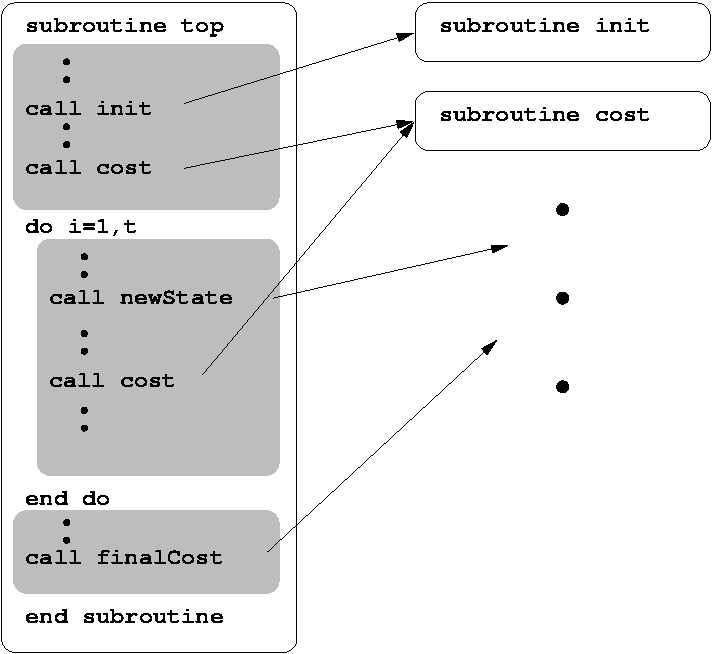
\includegraphics[height=4.3cm]{checkpointLoops}
\end{minipage}
&
\begin{minipage}{6cm}
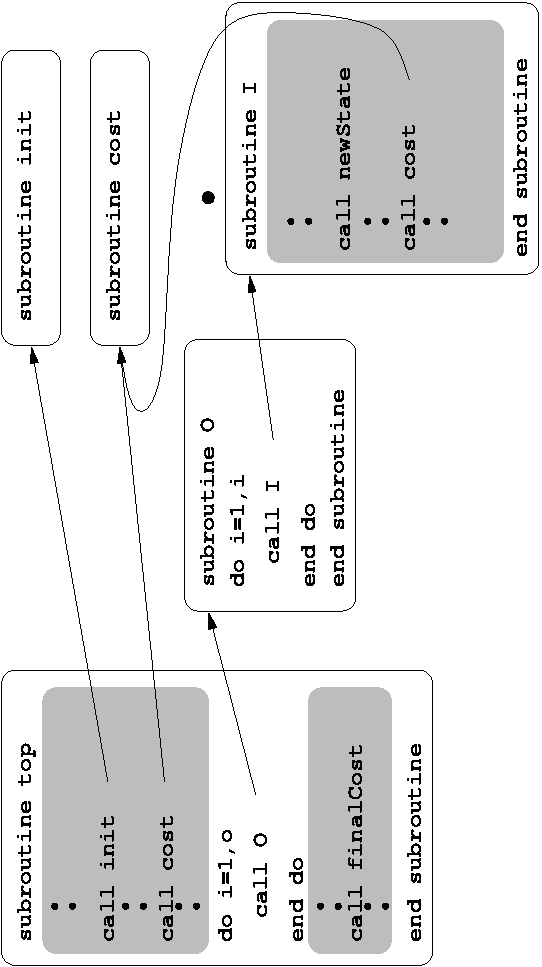
\includegraphics[width=4cm,angle=-90,origin=c]{checkpointLoopsNew2}
\vspace*{-2cm}
\end{minipage}\\
(a)& (b)
\end{tabular}
\caption{Modification of the original code (a) to allow 2 checkpointing levels (b)}\label{fig:checkpointLoops}
\end{figure}
Now we can describe the reversal scheme with the call tree shown in \reffig{fig:checkpointct}.
\begin{figure}
\begin{center}
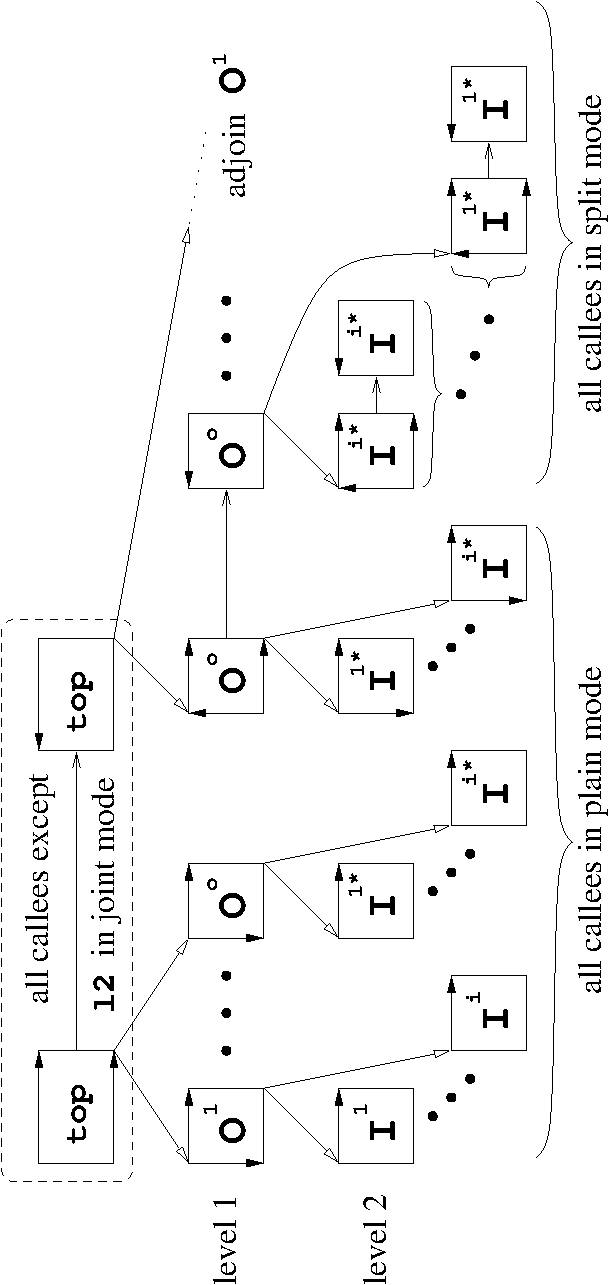
\includegraphics[width=4.3cm,angle=-90, origin=c]{swMode}
\vspace*{-3cm}
\end{center}
\caption{Checkpointing scheme, the {\tt .*} indicating {\tt .+(o-1)i}} \label{fig:checkpointct}
\end{figure}
The state changes can be encapsulated in four templates, one joint mode template for \code{top}
and all its callees except \code{O}, one for all callees of \code{I} and one  each for 
\code{O} and \code{I}.  
The collection of downloadable test problems contains the 
model and the four subroutine templates.
\reffig{fig:checkpointLoops}(b) shows the \code{cost} subroutine called from 
\code{I} as well as from \code{top}. 
However, according to \reffig{fig:checkpointLoops} we would need two versions of 
\code{cost}, one that as callee of \code{top} is reversed in joint mode and 
one as callee of \code{I} is reversed in split mode. In order to maintain 
the static reversal approach\footnote{
A dynamic reversal scheme is forthcoming.
}
one needs to duplicate \code{cost}.

% -----------------------------------------------------------------------------------------
\subsection{File I/O and Simple Loops}
The model code uses both the NetCDF library as well as 
the built in Fortran I/O during the initialization and 
output of results. Because  in the model computation 
no intermediate values are written and read during 
the model computation there is no loss of dependency information. 
However, the I/O can lead to problems, for instance 
when an activated array is initialized. The prevalent 
lack of type checking in Fortran may lead to setting 
the first half of the \code{\%v} and \code{\%d} values 
instead of setting all of the \code{\%v} values. 
This is a well known consequence of the active type 
implementation. While one could argue that the code should 
be generated to avoid reading or writing the derivative information
this is not always the actually desired behavior, in particular 
not if one reads or writes active intermediate variables. 
A simple and effective measure to circumvent this problem 
is let the initialization remain an external routine 
in which case \OpenADF\ will insert conversion routines 
for external subroutine parameters that are active at the 
call site. 
It should be noted that this approach does not work 
when instead of passing a parameter the external routine refers 
to active global variables.
  
Early tests showed a considerable amount of runtime and memory 
spent on taping array indices used in loops. 
The {\em simple} loop concept introduced in \refsec{sssec:cfgRevAlg}
is designed to eliminate much of this overhead. 
Not all loops within the given model code satisfy the conditions 
so as an additional step throughout the model code 
we identified the conformant loop constructs to 
the tool using the simple loop pragma. The resulting efficiency gain
was about a factor 4 in run time and more than a factor 10 in memory 
use.

% -----------------------------------------------------------------------------------------
\subsection{Results}
\reffig{fig:sensMap} shows as an example output a map of sensitivities of 
zonal volume transport through the Drake Passage 
to changes in bottom topography everywhere in a barotropic ocean model 
computed from the shallow water code by P. Heimbach.
\begin{figure}
\begin{center}
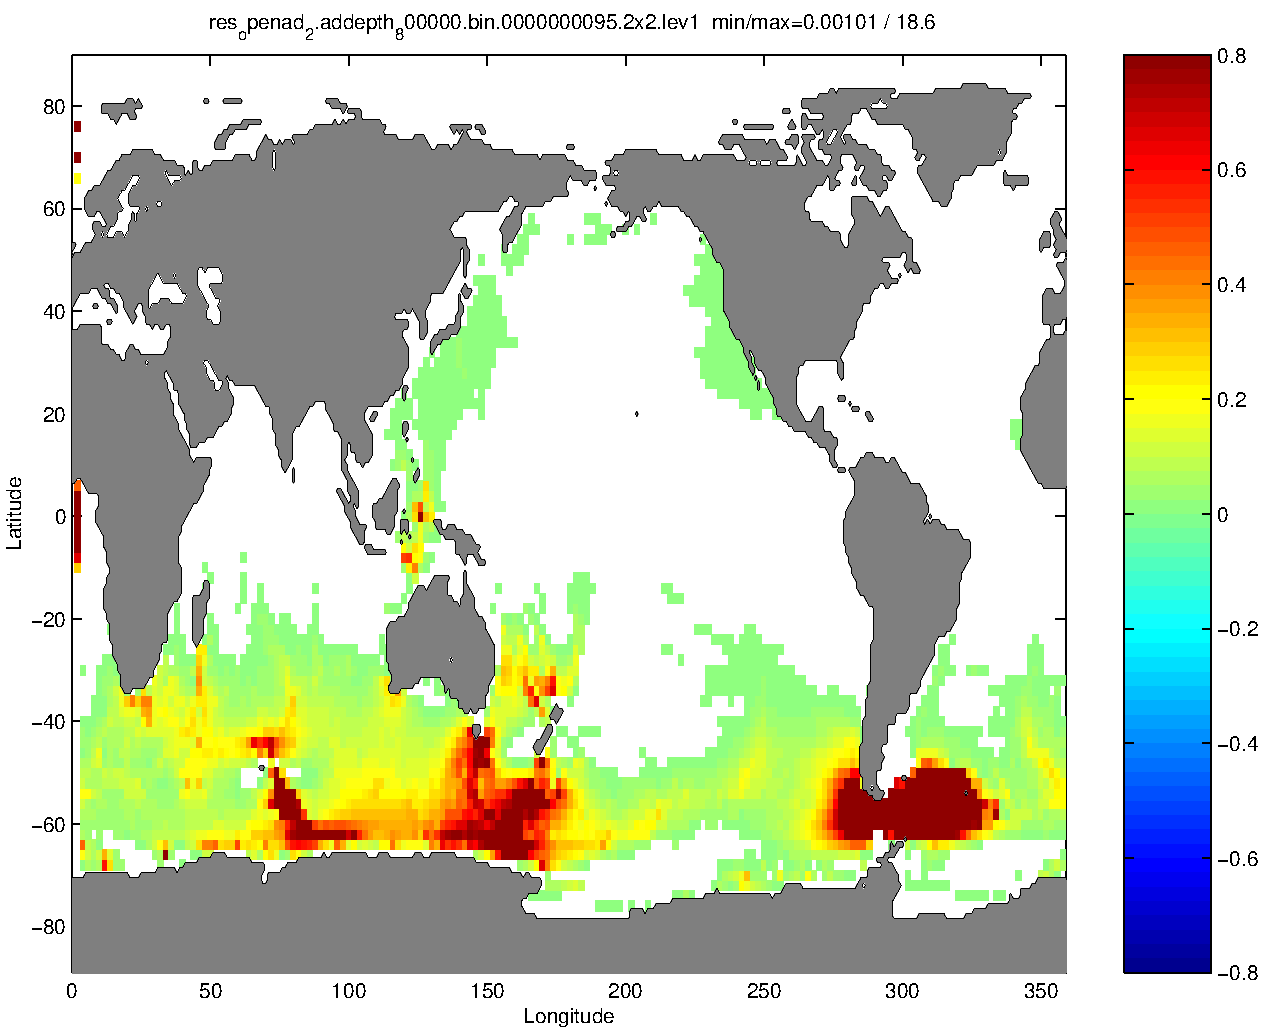
\includegraphics[height=6cm]{sensMap}
\end{center}
\caption{Sensitivity (gradient) map for $2\times 2$ degree resolution}\label{fig:sensMap}
\end{figure} 
The adjoint model generated with the current version of \OpenADF\ applied to the 
shallow water code achieves 
a run time that is only about 8 times that of  plain model computation.
We expect the ongoing development of \OpenADF, see also \refsec{chap:concl} to yield 
further efficiency gains.

% -----------------------------------------------------------------------------------------
\section{A Second Order Example}

{\color{red} candidate for removal, unless I get the fix in for the structure stuff}

% #########################################################################################
\chapter{Summary and Future Work}\label{chap:concl}

\OpenADF\ is an AD tool built on a language independent infrastructure with 
well-separated components. 
It 
allows developers to focus on various aspects of source-to-source 
transformation AD, including parsing and unparsing of different programming
languages, data and control flow analysis, and (semantic) transformation 
algorithms.
The components have well defined interfaces and intermediate stages 
are retained as either Fortran or XML sources. 
 
\OpenADF\ allows users a great amount of flexibility in the use of the code transformation
and permits interventions at various stages of the transformation process.
We would like to emphasize the fact that for large scale applications 
the efficiency of checkpointing and taping can be improved merely by 
modifying the implementation of the run time support, the template and inlining 
code. 
They are not conceived  to be just static 
deliverables of \OpenADF\ but rather are part of the 
interface accessible to the user.
It is not the intention to stop with a few prepackaged solutions as one 
would expect from a 
monolithic, black-box tool.  
True to the nature of an open source design, the interface is instead conceived as a 
wide playground for 
experimentation and improvement. 
Expanding on the schematic depiction 
of the tool workings in \reffig{fig:overview} we want to highlight 
the options to modify the transformation and the tool itself in \reffig{fig:pipelineIntervention} 
at different levels of complexity reaching from the casual user to 
actual coding work in the tool's components.    
\begin{figure}
\begin{center}
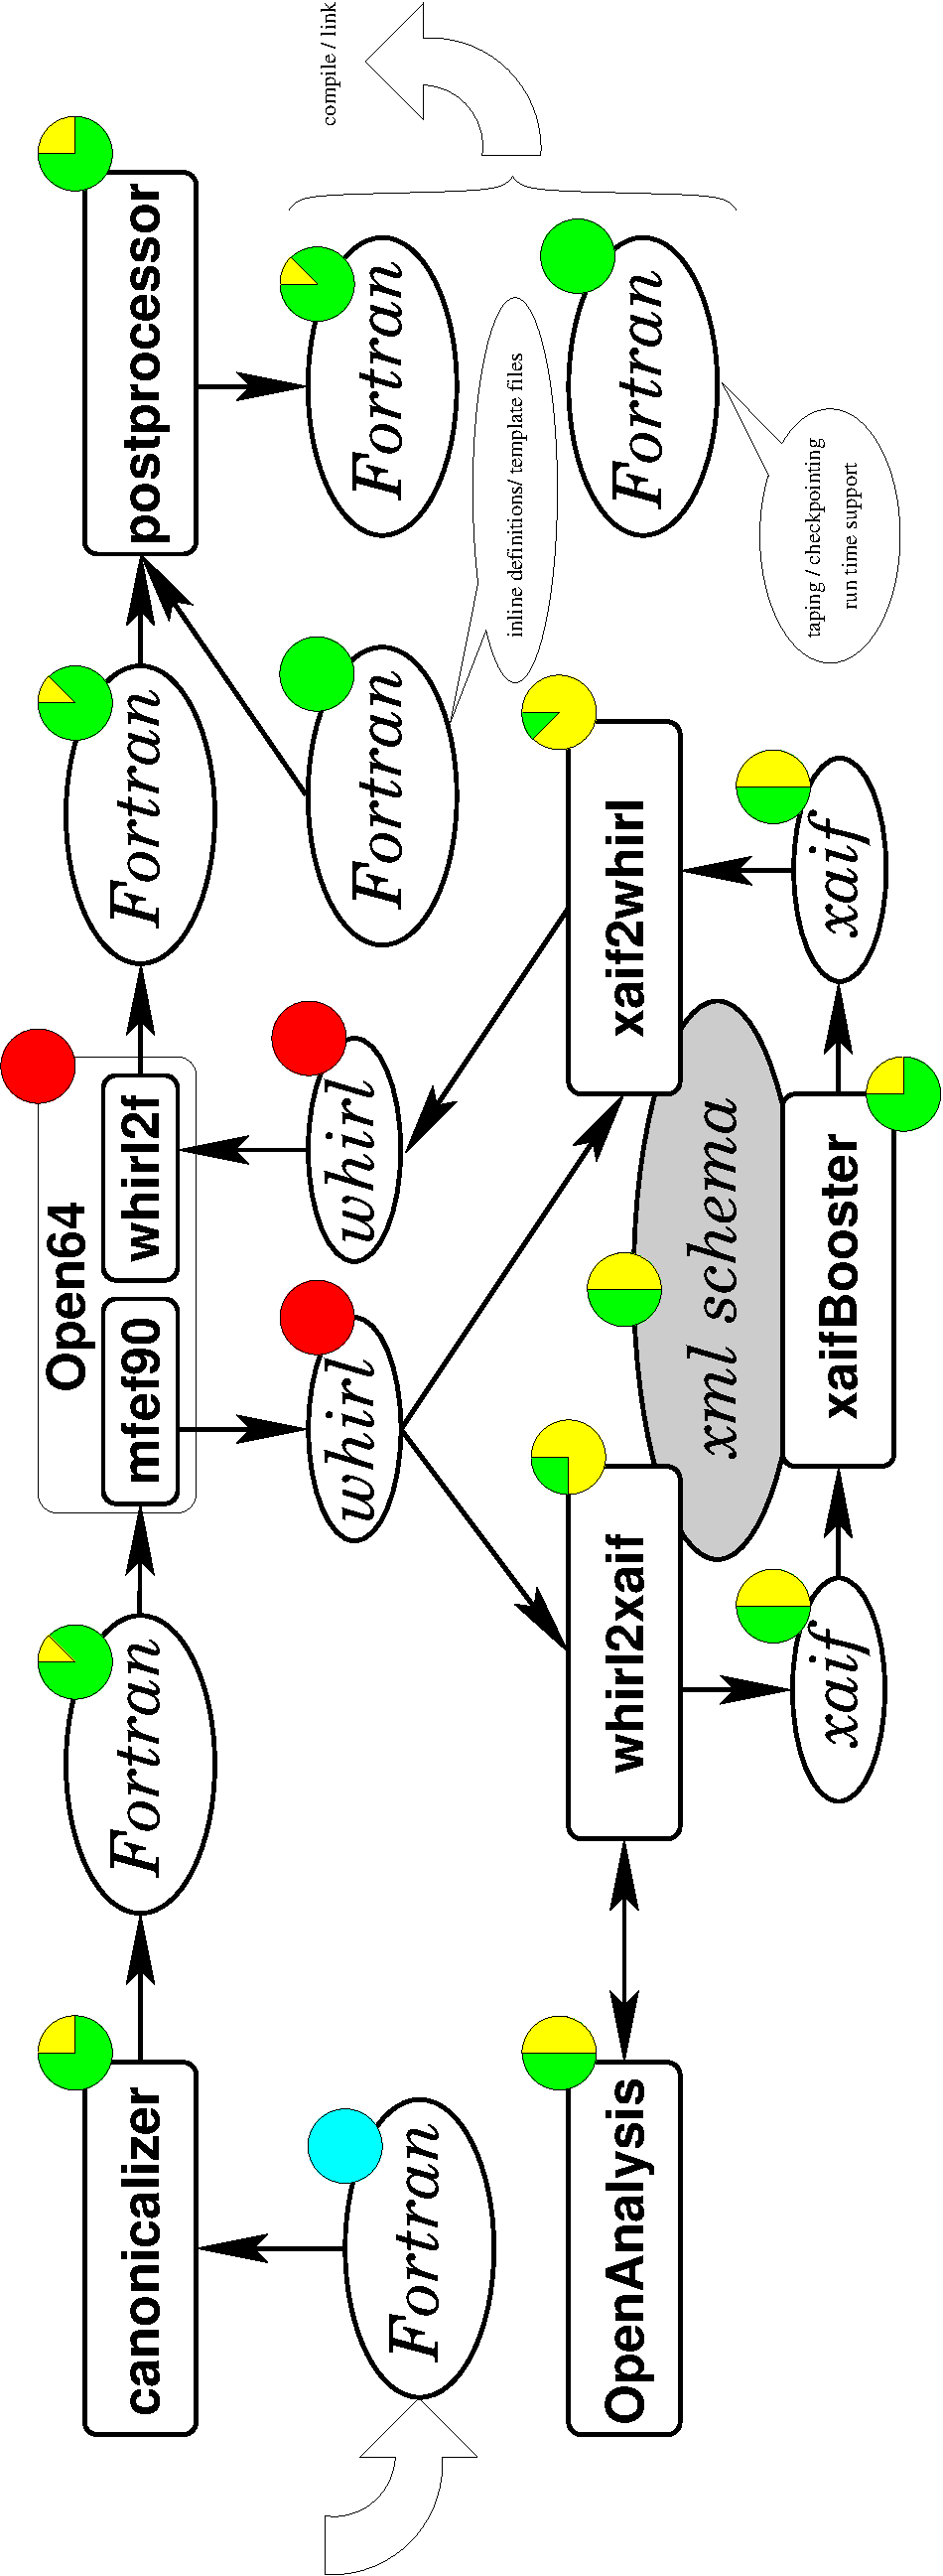
\includegraphics[angle=-90,width=\textwidth,origin=c]{overview2}
\end{center}
\vspace*{-4cm}
\caption{Levels of complexity for modifications}\label{fig:pipelineIntervention}
\end{figure} 
As part of using \OpenADF\ for different applications we see a growing number of 
variations to the  transformation and run time support implementations available 
to the user.

Aside from the plain AD tool aspect the intention of the 
underlying \OpenAD\  framework is to 
provide the AD community with 
an open, extensible, and easy-to-use platform for research and development
that can be applied across programming languages.
Tools that have a closer coupling with a language-specific, internal representation
have the potential to make the exploitation of certain language features easier. 
Consequently we do not expect \OpenADF\ to obsolete existing source transformation
tools such as  
the differentiation-enabled NAG Fortran 95 
compiler,
\footnote{\code{http://www.nag.co.uk/nagware/research/ad\_overview.asp}} 
TAF,\footnote{\code{http://www.FastOpt.de}} 
or TAPENADE.\footnote{\code{http://tapenade.inria.fr:8080/tapenade/index.jsp}} 
Rather it is to
complement these tools by providing well-defined APIs to an open internal 
representation that can be used by a large number of AD developers.
Users of AD technology will benefit from the expected
variety of combinations of front-ends and algorithms that is made possible
by \OpenADF.

As with any software project there is ample room for improvement.
The robustness of the tool, in particular the coverage of 
some specific language features, often is of concern to first 
time users. While robustness is not to be disregarded, it is clearly 
not a research subject and as such cannot be made the major 
objective of a development project in an academic setting. 
Robustness issues affect mostly the language dependent components 
and the contributing parties undertake a considerable effort to 
address concerns common to many applications. Many issues specific 
to a particular input code can be addressed by minor adjustments 
which often happen to reflect good coding practices anyway. 
Take for example a change away from 
\code{goto - label} to a well structured control flow. 
While we plan to  implement code that handles 
unstructured control flow at some point, the corresponding adjoint  will always
be less efficient than the respective structured equivalent and an 
automatic transformation to structured control flow is somewhat beyond the scope
of an AD tool.

We are concerned with changes that affect many applications and yield 
improved efficiency of the adjoint code.
Currently the most important items on the development list are the
support for vector intrinsics and the handling of allocation/deallocation cycles 
during the model computation for the generation of an adjoint model.
Because the tool provides a variety of options to the user we are also 
working on collecting data for efficiency estimates that permit 
an informed choice between the code transformation options. 
Ongoing research in AD algorithms, in particular dynamic call 
graph reversal, more efficient control flow reversal and 
improved elimination techniques in the computational graphs will 
be incorporated into \OpenAD. 

% #########################################################################################
\chapter*{Appendix}
\begin{table}
  \tiny
  \begin{center}
    \begin{tabular}{ll}
      {\tt Makefile} & the top level {\tt Makefile}\\
      {\tt utils/} & utility classes (debugging, generic traversal, etc.)\\
      {\tt tools/}  & code generator supporting \xaif\ parser \\
      {\tt boostWrapper/}& wrapper classes for the boost graph library \\
      {\tt system/} & all basic data structures, \xaif\ (un)parsing, \refsec{ssssec:readWriteXaif}\\
      {\tt algorithms/}& see the subdirectories below\\
      \quad{\tt CodeReplacement} & support library for subroutine templates\\
      \quad{\tt CrossCountryInterface} & support library for elimination strategies, \refsec{sssec:BBPreacc}\\
      \quad{\tt DerivativePropagator} & support library for Jacobian vector products\\
      \quad{\tt InlinableXMLRepresentation } & support library for inlinable subroutine calls\\ 
      \quad{\tt Linearization} & Linearization transformation, \refsec{sssec:linearization}\\ 
      \quad{\tt BasicBlockPreaccumulation} & elimination with \angel\ and \\
      & preaccumulation at the \basicblock\ level, \refsec{sssec:BBPreacc}\\
      \quad{\tt  MemOpsTradeoffPreaccumulation} & as above but with different heuristics than \angel\\
      \quad{\tt ControlFlowReversal} & control flow graph reversal\\
      \quad{\tt BasicBlockPreaccumulationReverse } & adjoint code\\
      \quad{\tt BasicBlockPreaccumulationTape } & taping code supporting adjoint, \refsec{sssec:bbTA}\\
      \quad{\tt BasicBlockPreaccumulationTapeAdjoint } & reverse sweep portion supporting adjoint,\refsec{sssec:bbTA}\\
    \end{tabular}
  \end{center}
  \caption{Directory structure in \xaifBooster}\label{tab:dirStruct}
\end{table}
\bibliographystyle{plain}
\bibliography{openad}
\include{index}
  \addcontentsline{toc}{chapter}{Index}
\end{document}
